\documentclass[11pt, a4paper, twocolumn, copyright, goog]{google}

\usepackage{iftex}
\ifXeTeX
\usepackage{fontspec}
\usepackage{xeCJK}
\defaultfontfeatures{Ligatures=TeX}
\setmainfont{Times New Roman}
\setsansfont{Arial}
\setmonofont{Menlo}
\IfFontExistsTF{Songti SC}{
    \setCJKmainfont{Songti SC}
}{
    \IfFontExistsTF{STSong}{
        \setCJKmainfont{STSong}
  }{
    \setCJKmainfont{STHeiti}
  }
}
\fi

\usepackage[authoryear, sort&compress, round]{natbib}
\bibliographystyle{abbrvnat}


% 如果不需要可移除
% \keywords{paper template, tools}/
% \paperurl{https://arxiv.org/abs/123}

% 如果不需要 logo 可注释掉
\uselogo{go} 

% 论文标题
\title{关于在自适应优化器中掩码更新的惊人有效性}

% 如果不希望添加通讯作者，可省略该选项。
\correspondingauthor{taejong.joo@northwestern.edu, cheolmin@google.com}
% \correspondingauthor{}


% 若有内部论文编号可填写
\reportnumber{} % 若不适用则留空

% 可为报告指定日期。
% 若不需要可注释，或不适用时留空。
\renewcommand{\today}{2026-02-16}

\usepackage{color, colortbl}
\definecolor{Gray}{gray}{0.9}



\newcommand{\change}[1]{{\red{magenta} #1}}



\usepackage{amsmath}
\usepackage{amssymb}
\usepackage{mathtools}
\usepackage{amsthm}

\usepackage{enumitem}


\input{math_commands}


\usepackage{xcolor} % http://www.ctan.org/tex-archive/macros/latex/contrib/xcolor


\usepackage[capitalize,noabbrev]{cleveref}

%%%%%%%%%%%%%%%%%%%%%%%%%%%%%%%%
% 定理环境
%%%%%%%%%%%%%%%%%%%%%%%%%%%%%%%%
\theoremstyle{plain}
\newtheorem{theorem}{定理}
\newtheorem{proposition}[theorem]{命题}
\newtheorem{lemma}[theorem]{引理}
\newtheorem{corollary}[theorem]{推论}
\theoremstyle{definition}
\newtheorem{definition}[theorem]{定义}
\newtheorem{assumption}[theorem]{假设}
\theoremstyle{remark}
\newtheorem{remark}[theorem]{注记}


\usepackage{xcolor}
\usepackage{graphicx}


% 尝试让 hyperref 与 algorithmic 配合更好：
% \usepackage{algorithm}
% \usepackage{algpseudocode}
% \newcommand{\theHalgorithm}{\arabic{algorithm}}

% 作者与机构可按需扩展。建议按下方方式标注共同一作。
\author[1,*]{Taejong Joo}
\author[2]{Wenhan Xia}
\author[2]{Cheolmin Kim}
\author[2]{Ming Zhang}
\author[2]{Eugene Ie}

% \affil 必须放在 \author[] 之后
\affil[1]{西北大学}
\affil[2]{Google}
\affil[*]{该工作完成于作者在 Google 担任学生研究员期间。}



\begin{abstract}
大语言模型（LLM）的训练几乎完全依赖于稠密自适应优化器，并且其预条件器日益复杂。
我们对这一范式提出挑战：我们表明，随机掩码参数更新可以非常有效，且 RMSProp 的一个掩码变体持续优于近期最先进优化器。
我们的分析揭示，随机掩码会诱导一种依赖曲率的几何正则化，从而平滑优化轨迹。 
受此发现启发，我们提出了 \textbf{\underline{M}omentum-\underline{a}ligned \underline{g}radient \underline{ma}sking (Magma)}，其利用动量-梯度对齐来调制掩码更新。
大规模 LLM 预训练实验表明，Magma 是一种简单的可即插即用替代方案，在几乎不增加计算开销的情况下带来稳定增益。
特别地，在 1B 模型规模上，相较 Adam 与 Muon，Magma 分别将困惑度降低超过 19\% 与 9\%。
\end{abstract}



\begin{document}

\maketitle

\section{引言}
反向传播中一次反向传递即可得到稠密梯度 \citep{rumelhart1986learning}，从而支持高效的并行参数更新。 
这种效率使 Adam \citep{kingma2014adam} 等稠密自适应优化器成为大规模 LLM 训练的事实标准。 
相比之下，这种对稠密梯度的依赖与稀疏更新策略（如坐标下降）之间存在结构性不匹配 \citep{nesterov2012efficiency,wright2015coordinate,nutini2017let}。 
因此，尽管稀疏方法在 LLM 训练常见的高度非光滑优化问题上表现强劲，它们在该场景中仍很少被采用。



{\begin{algorithm}[tb]
\caption{\colorbox{blue!30}{\pmb{SkipUpdate}} 与 \colorbox{red!30}{\pmb{Magma}}。}
\label{alg:magma_pseudocode}
\footnotesize
  \begin{algorithmic}
    \STATE {\bfseries 输入:} 参数 $\{ \theta_t^{(b)}\}_{b=1}^{B}$，随机梯度 $\{ \vg_t^{(b)}\}_{b=1}^{B}$，来自基础优化器的更新 $\{ \Delta_t^{(b)}\}_{b=1}^{B}$，一阶动量估计 $\{\mu_{t}^{(b)}\}_{b=1}^{B}$
    \FOR{每个块 $b \in [B]$}
        \STATE \colorbox{blue!30}{$s_t^{(b)} = 2$ \quad \pmb{(SkipUpdate)}}
        \STATE \colorbox{red!30}{%
        \parbox{0.65\linewidth}{%
        $\tilde{s}_t^{(b)} =
        \sigmoid(\mathrm{cossim}(\mu_t^{(b)},\vg_t^{(b)})/\tau)$\\
        $s_t^{(b)} =
        0.9 s_{t-1}^{(b)} + 0.1 \tilde{s}_t^{(b)}$
        \quad \pmb{(Magma)}%
        }}
        \STATE $m_{t}^{(b)} \sim \mathrm{Bernoulli}(0.5)$
        \STATE $\theta_{t+1}^{(b)} = \theta_t^{(b)} -  s_t^{(b)} m_{t}^{(b)} \Delta_t^{(b)} $
    \ENDFOR
  \end{algorithmic}
\end{algorithm}
}


\begin{figure}
\vskip -0.1in
\begin{center}
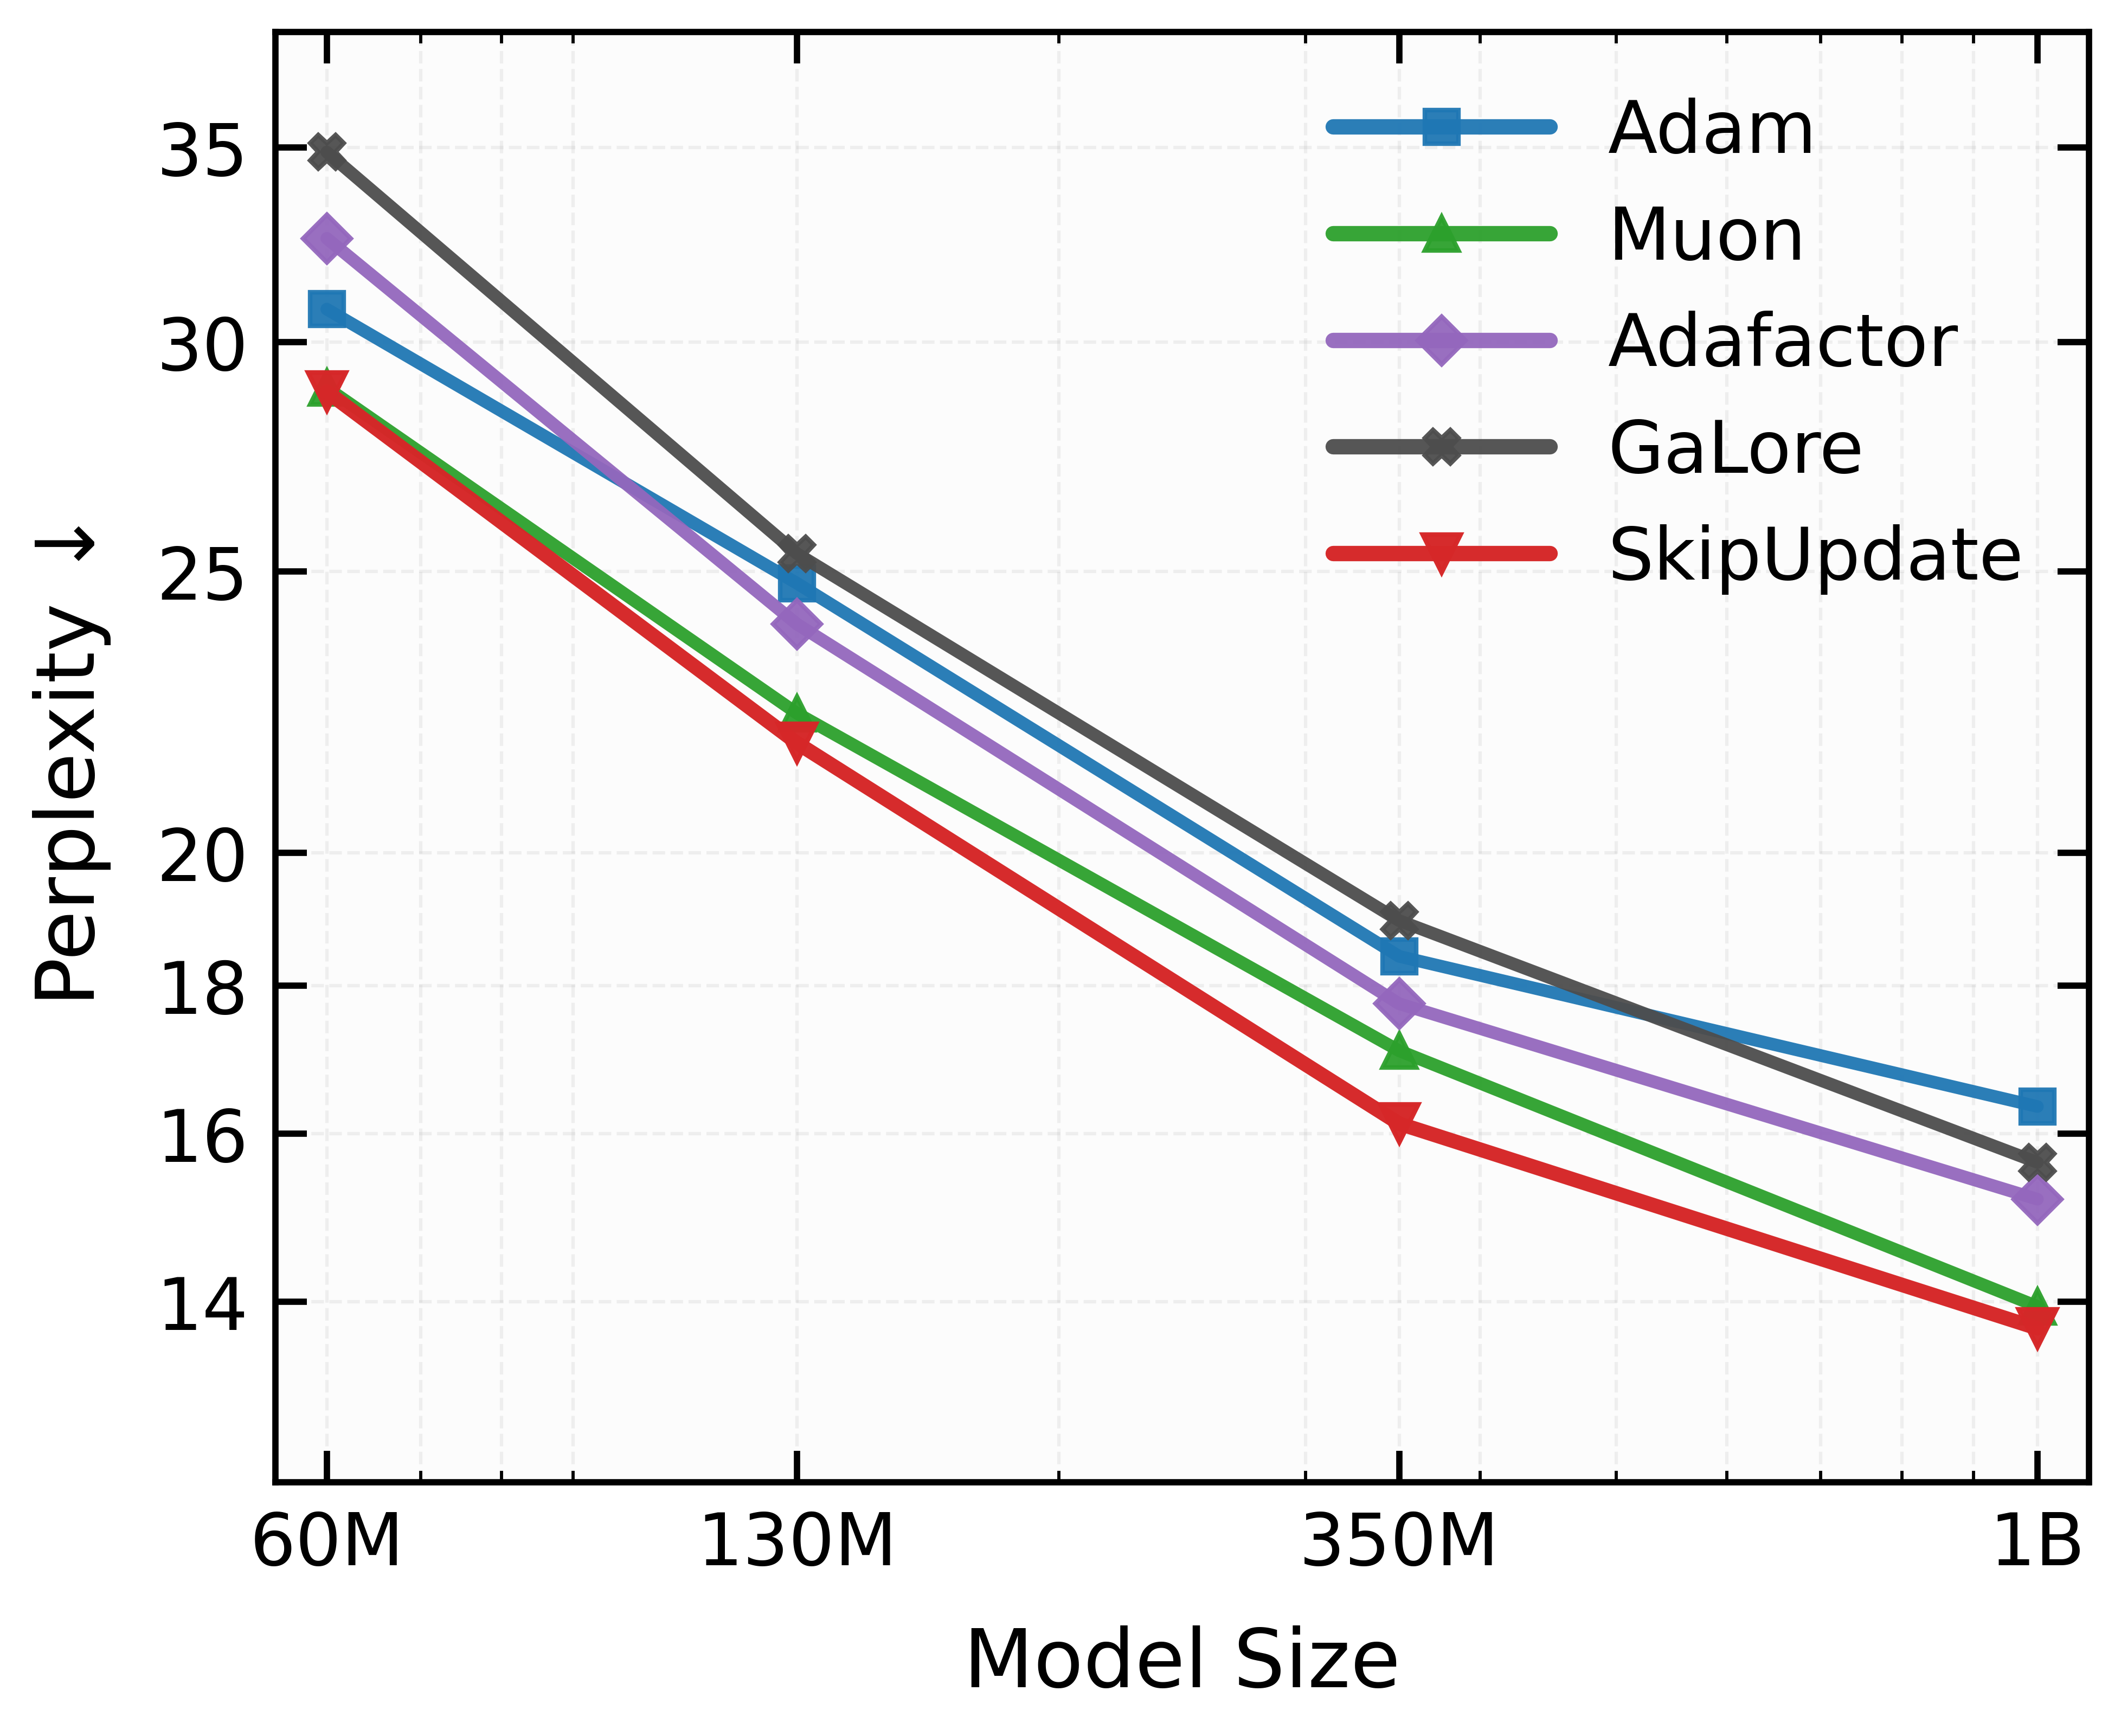
\includegraphics[width=0.85\columnwidth]{figs/magma_fig1.png}
\end{center}
\vskip -0.15in
\caption{
\textit{
C4 上不同模型规模的预训练性能。}
尽管丢弃了一半更新，SkipUpdate 仍显著优于最先进的稠密优化器。
}
\label{fig1:observation_mask}
\vskip -0.2in
\end{figure}


在本文中，我们通过一个反直觉的经验发现挑战这一主流范式：\emph{随机掩码梯度更新能够显著提升优化性能}。
具体而言，我们研究了 RMSProp \citep{hinton2012rmsprop} 的一个变体：在每次迭代中按伯努利分布对整个参数块进行随机掩码。若某块被掩码，则该步跳过其参数更新；但动量估计仍保持稠密更新，且对保留下来的更新进行适当重缩放以保持无偏性（见算法 \ref{alg:magma_pseudocode} 中的 SkipUpdate）。
从经典收敛分析视角看，这类随机掩码会因更新噪声增大而导致更差的最坏情形收敛保证（见 \S \ref{sec:convergence_analysis}）。此外，每个参数在每次迭代中实际收到的更新更少，而通过反向传播计算梯度的成本并未变化。
然而，尽管丢弃了一半更新，SkipUpdate 仍在各模型规模上持续优于稠密优化器（包括融合精细曲率信息的最新 SOTA 优化器 Muon \citep{jordan2024muon}，见图~\ref{fig1:observation_mask}）。




为解释 SkipUpdate 的有效性，我们分析其几何正则化效应。
具体地，我们证明按块掩码会诱导依赖曲率的几何正则化：对每个参数块内与损失陡峭方向对齐的更新进行惩罚。
这一效应平滑了优化轨迹，并使算法偏向损失景观中更平坦的区域；经验上，这类区域与深度网络更好的泛化相关 \citep{hochreiter1997flat,keskar2016large,jastrzkebski2017three}。
重要的是，该正则化并非来自显式曲率计算，而是由更新规则中的随机噪声隐式产生。


我们进一步探究：能否利用自适应优化器中已有信息，使随机掩码更有效。
我们发现，依据随机梯度与一阶动量估计之间的余弦相似度来调制掩码更新，可带来显著收益。
该机制通过抑制与梯度累积方向不一致的更新，优先保留与动量一致的更新。
由此得到 \textbf{\underline{M}omentum-\underline{a}ligned \underline{g}radient \underline{ma}sking (Magma)}，其稳定优于自适应优化器与 SkipUpdate。
值得注意的是，Magma 的优势随模型规模增大而增强，这与“大模型具有更具挑战性的优化景观、需要更强几何正则化”这一现象一致。


我们的贡献如下：
\underline{\textbf{\textit{(i) 方法层面：}}} Magma 是一个简单的优化器封装器，在不增加计算成本的前提下，提升了 Transformer 特殊损失景观下的训练稳定性与泛化能力；
\underline{\textit{\textbf{(ii) 理论层面：}}} 我们证明随机梯度掩码会诱导朝向更平坦轨迹的几何正则化，从而降低曲率尖锐性与梯度噪声；
\underline{\textbf{\textit{(iii) 实证层面：}}} 我们在多种预训练场景下验证了其相较最先进优化器的一致性能增益。



% ========================================================================
% ========================================================================
% ========================================================================
%         理论分析
% ========================================================================
% ========================================================================
% ========================================================================


\section{将更新掩码视为一种正则化} \label{subsec:implicit_reg}

\textbf{记号。}
记 $\theta_t$ 为迭代 $t$ 时的模型参数，其可划分为 $B$ 个互不相交的块 $\{ \theta_t^{(b)} \}_{b=1}^B$。 
在全文中，我们将每个块视为独立参数单元。
记 $\nabla_b l(\theta)$ 为损失 $l$ 关于 $\theta^{(b)}$ 的梯度。$t$ 时刻 $l(\cdot)$ 的随机梯度记为 $\vg_t \triangleq \{ \vg_t^{(b)} \}_{b=1}^B$。
$\mathbf{H}_{bb'}(\theta_t)$ 表示 Hessian $\nabla^2 l(\theta_t)$ 的 $(b,b')$ 分块。 
令 $(\gF_t)_{t \geq 0}$ 为一个滤过，使得 $\theta_t$ 对 $\gF_t$ 可测，且 $\E_t[\cdot] \triangleq \E [\cdot | \gF_t]$。 

\textbf{背景：自适应优化器与动量估计。}
自适应优化器通过过去梯度的运行统计（通常是对角或块对角预条件）来调节更新幅度。 
给定学习率 $\eta_t$，其更新形式为 $\theta_{t+1}^{(b)} = \theta_t^{(b)} - \eta_t \mD_t^{(b)} \vg_t^{(b)},$
其中 $\mD_t^{(b)}$ 是正定（通常对角）矩阵，编码逐参数或逐块的自适应调节。 
主流自适应优化器主要差异在于 $\mD_t^{(b)}$ 的构造方式，或将 $\vg_t^{(b)}$ 替换为更稳定的梯度估计器；这通常涉及两类梯度信息的滑动平均。一阶动量估计为 $\mu_{t}^{(b)} = \beta_1 \mu_{t-1}^{(b)} + (1 - \beta_1) \vg_t^{(b)}$，二阶动量估计跟踪梯度平方 $\vv_t^{(b)} = \beta_2 \vv_{t-1}^{(b)} + (1 - \beta_2) (\vg_t^{(b)})^2,$ 其中 $\beta_1, \beta_2 \in (0,1)$ 为常数。
RMSProp 使用 $\mD_t^{(b)} \approx \text{diag} (\vv_t^{(b)})^{-1/2}$。



\textbf{主要结论。}
在迭代 $t$，令 $\Delta_t = (\Delta_t^{(1)},\ldots,\Delta_t^{(B)})$ 表示来自基础优化器的按块更新方向（例如自适应优化器中的 $\eta_t \mD_t^{(b)} \vg_t^{(b)}$）。 
SkipUpdate 引入独立伯努利随机变量 $\{m_{t}^{(b)}\}_{b=1}^B$，其中 $m_{t}^{(b)} \sim \mathrm{Bernoulli}(p)$，生存概率为 $p \in (0,1]$。
随后对更新施加随机按块掩码： 
\begin{equation} \label{eq:rsu_def}
    \tilde{\Delta}_t^{(b)} =  s_t^{(b)} m_{t}^{(b)}\Delta_t^{(b)} , 
\qquad b = 1,\ldots,B,
\end{equation}
得到 $\tilde{\Delta}_t \triangleq (\tilde{\Delta}_t^{(1)},\ldots,\tilde{\Delta}_t^{(B)})$。我们设 $s_t^{(b)} = 1/ p$ 以保证掩码更新无偏，即 $\E_t [ \tilde{\Delta}_t^{(b)} ] = \Delta_t^{(b)}$。



尽管随机掩码保持了期望更新不变，但它从根本上改变了优化动力学的高阶行为。
在下述命题中（证明见附录 \ref{appx:proof_prop1}），我们证明 SkipUpdate 在期望损失下降中诱导了一个依赖曲率的项。

\begin{proposition}[] \label{lemma:implicit_reg}
在条件 $\gF_t$ 下，SkipUpdate（见 \eqref{eq:rsu_def}）的期望损失满足
\begin{multline} \label{eq:implicit_reg}
    \mathbb{E}_t\left[l(\theta_t-\tilde{\Delta}_t) \right] = l(\theta_t-\Delta_t) + \\
    \sum_{b=1}^B \frac{1-p}{2p} (\Delta_t^{(b)})^\top  \mathbf{H}_{bb}(\theta_t) \Delta_t^{(b)}
    + \gO(\sum_{b=1}^B \|\Delta_t^{(b)}\|^3).
\end{multline}
\end{proposition}


项 $\gR_t^{(b)} \triangleq \frac{1-p}{2p} (\Delta_t^{(b)})^\top \mathbf{H}_{bb}(\theta_t) \Delta_t^{(b)}$ 可自然解释为一种\emph{几何正则器}。 
它衡量了沿更新方向 $\Delta_t^{(b)}$ 的局部损失曲率，并大致按生存概率的倒数加权。 
由于大正曲率方向对应损失的急剧上升，最小化更新后期望损失会隐式抑制各块中与高曲率方向对齐的更新。 


这种块结构正则化与 Transformer 的经验几何特征高度契合：其 Hessian 通常呈现显著块对角结构 \citep{zhang2024transformers,kunstner2024heavy,ormaniec2024does}。
在该几何下，主导曲率交互主要发生在块内。 
因此，命题 \ref{lemma:implicit_reg} 中的块级二次惩罚形成了有原则的二阶正则化，使优化偏向更平坦的损失区域。长期以来，这类平坦极小值与更好泛化相关 \citep{hochreiter1997flat,keskar2016large}，也是 sharpness-aware 优化方法的目标 \citep{foret2020sharpness}。




\textbf{为何稠密动量更新很重要。}
在算法 ~\ref{alg:magma_pseudocode} 中，即便参数更新被掩码，动量状态仍进行稠密更新。 
这与近期子空间优化方法 \citep{pan2024lisa,zhao2024galore,luo2024badam} 不同，后者仅在选中坐标上同时更新参数与辅助状态。
例如，GaLore \citep{zhao2024galore} 通过梯度主奇异向量选择坐标，并在固定批次区间内更新这些坐标。
尽管这可降低优化器内存，但它会反复优化次优坐标子集，这与经典坐标下降洞见相悖 \citep{nesterov2012efficiency,nutini2017let}。
此外，在现代 LLM 训练中，内存瓶颈通常由激活而非参数或优化器状态主导，因此显著内存节省并不总能保证 \citep{zhang2024revisiting,shamshoum2025compact}。



进一步地，由于惰性更新机制，SkipUpdate 实际上可形成对真实动量的降方差估计器，从而产生更稳定的搜索方向。
因此，如图 \ref{fig:dense-vs-sparse-momentum-update} 所示，相比内存高效子空间优化器中的稀疏动量更新，稠密动量更新具有更高稳定性和更好泛化。




\textbf{结构化掩码的影响。}
命题 \ref{lemma:implicit_reg} 表明，掩码粒度决定了诱导曲率正则器的结构；粒度越细，跨坐标交互越被消除。
例如，逐元素掩码仅惩罚 Hessian 对角项，其正则项为 $\sum_{b=1}^B \sum_{i=1}^{\textrm{dim}(b)} \frac{1-p}{2p} \{ \Delta_t^{(b)} \}_{i}^2   \{ \mathbf{H}_{bb}(\theta_t) \}_{i,i},$ 其中 $\textrm{dim}(b)$ 为块 $b$ 的维度。
有趣的是，在 C4 上进行 130M Llama 预训练时，SkipUpdate 在不同掩码粒度下困惑度相近——21.78（按列）、21.73（按元素）与 21.81（按块）——且均显著优于 RMSProp 基线（22.64）。
我们推测，这种近似等价反映了对角预条件难以充分利用块内稠密曲率，因此更细粒度掩码的实际收益有限。
因此，我们采用按块掩码，因为跳过整个块可带来更优的计算性质与操作裁剪效率。



% ========================================================================
% ========================================================================
% ========================================================================
%         方法
% ========================================================================
% ========================================================================
% ========================================================================




\section{动量对齐更新掩码} \label{sec:mainsection}
SkipUpdate 在所有块上施加同质掩码。
然而，Transformer 参数表现出明显异质性，例如 Hessian 谱差异显著 \citep{zhang2024transformers}、梯度方差差异显著 \citep{orvieto2025search}。 
这种异质性会强烈影响优化动力学，因此需要更精细的块自适应掩码策略，同时保持与现代自适应优化器的无缝兼容。

在随机优化中，跨迭代保持一致的梯度分量通常携带有效优化信号，而快速波动的分量往往由随机噪声主导 \citep{polyak1964some,riedmiller1993direct,bottou2018optimization}。
此外，近期工作从在线变分推断视角解释了动量估计 \citep{orvieto2025search}。在该视角下，负对齐概率满足
$\mathbb{P}(\mu^\top g < 0) = \Phi \left(-\frac{\|\mu\|}{\sigma} \right),$ 且随信噪比 $\|\mu\|/\sigma$ 指数衰减。
因此，负对齐事件代表统计上异常的波动，可作为识别不稳定更新的自然信号。
这促使我们采用\emph{动量-梯度对齐}作为调制更新幅度的原则性准则。



基于上述洞见，我们提出 Magma，通过块级动量-梯度对齐控制掩码过程。
具体地，对迭代 $t$ 的每个块 $b$，Magma 计算对齐分数 $\tilde{s}_t^{(b)} \in (0,1)$：
\begin{equation} \label{eq:masking_prob}
    \tilde{s}_t^{(b)} = \sigmoid\left( \textrm{cossim}(\mu_t^{(b)}, \vg_t^{(b)}) / \tau \right),
\end{equation}
其中 $\mu_t^{(b)}$ 是一阶动量估计，$\tau > 0$ 为温度参数，$\textrm{cossim}(\cdot, \cdot)$ 为余弦相似度。 
我们采用余弦相似度是因为其尺度不变性，这在 LLM 训练中尤为有效——梯度范数在不同参数块与不同迭代间变化都很大 \citep{huang2025spam, wen2025sron}。 


随后，Magma 根据对齐分数 $s_t^{(b)}$ 调制含噪（掩码）更新，更新规则为 $\tilde{\Delta}_t^{(b)} =  s_t^{(b)} m_{t}^{(b)}\Delta_t^{(b)}, \; b = 1,\ldots,B,$ 其中 $s_t^{(b)} = 0.9 s_{t-1}^{(b)} + 0.1 \tilde{s}_t^{(b)}$ 为指数滑动平均。
因此，Magma 会通过较大的 $s_t^{(b)}$ 鼓励连贯优化轨迹，并通过较小的 $s_t^{(b)}$ 缓解振荡更新。 
我们强调，Magma 是一个可即插即用的封装器：仅将 $s_t^{(b)} m_{t}^{(b)}$ 乘到（自适应）优化器产生的既有更新方向 $\Delta_t^{(b)}$ 上，不引入额外内存或计算开销。
因此，实践者可在现有训练流水线中以极少代码改动、且无需额外资源地部署 Magma。

Cautious Optimizer \citep{liang2024cautious} 与 MGUP \citep{chang2025mgup} 也基于类似思想：对随机梯度与一阶动量估计符号相反的参数更新进行掩码或衰减。类似地，RPROP \citep{riedmiller1993direct} 依据梯度符号的时间一致性自适应步长。
但与 Magma 不同，这些方法缺乏结构化随机掩码，因此不会诱导 \S \ref{subsec:implicit_reg} 中建立的依赖曲率几何正则化。 


乘以对齐分数（阻尼）会给掩码更新引入偏差，但可显著提升训练稳定性（见附录图 \ref{fig:dense-vs-sparse-momentum-update}）。我们也测试了无偏替代方案，例如将 $\tilde{s}_t^{(b)}$ 用作生存概率并以 $1/\tilde{s}_t^{(b)}$ 重缩放，但它们始终导致训练不稳定。为 Magma 设计稳定且无偏的掩码机制仍是重要未来方向。




% ========================================================================
% ========================================================================
% ========================================================================
%         实验
% ========================================================================
% ========================================================================
% ========================================================================
\section{实验}

\begin{table}[t]
\caption{C4 数据集上的 Llama 2 预训练结果。 
我们报告了四个模型规模（60M 至 1B）的验证困惑度。$\dagger$ 表示结果来自 \citet{li-etal-2025-taming}；其余结果为我们复现。RMSProp 在学习率搜索范围内对 1B 模型发生发散。}
\centering
\resizebox{\columnwidth}{!}{%
\begin{tabular}{lcccc}
\toprule
\textbf{方法} & {\textbf{60M}} & {\textbf{130M}} & {\textbf{350M}} & {\textbf{1B}} \\
\midrule 
Adam & 30.79 & 24.77 & 18.42 & 16.35 \\ 
C-Adam & 29.70 & 23.59 & 18.58 & 15.92 \\
Adam+SGG$\dagger$ & 30.31 & 22.18 & 17.28 & 14.30 \\ 
\rowcolor{Gray} Adam+Magma & \pmb{29.09} & \pmb{22.08} & \pmb{16.41} & \pmb{13.71} \\
\midrule 
LaProp & 29.98 & 23.07 & 18.56 & 16.38 \\
\rowcolor{Gray} LaProp+Magma & \pmb{29.05} & \pmb{22.16} & \pmb{16.37} & \pmb{13.82} \\
\midrule 
Adafactor$\dagger$  & 32.57 & 23.98 & 17.74 & 15.19 \\ 
APOLLO$\dagger$  & 31.55 & 22.94 & 16.85 & 14.20 \\ 
APOLLO+SGG$\dagger$  & 30.18 & 22.52 & 16.54 & 13.95 \\ 
Muon$\dagger$ & 28.93 & 22.34 & 17.09 & 14.52 \\
RMSProp & 29.29 & 22.64 & 17.47 & - \\
\midrule 
\rowcolor{Gray} RMSProp+Magma & \pmb{28.55} & \pmb{21.66} & \pmb{16.16} &  \pmb{13.19} \\ 
\bottomrule
\end{tabular}
}
\label{table:benchmark_c4}
\end{table}



\subsection{Llama 预训练}  \label{subsec:pre-training-llms}

我们在 C4 数据集 \citep{raffel2020exploring} 上报告 Llama 2 预训练结果，模型规模覆盖 60M、130M、350M 与 1B，并遵循 \citet{zhao2024galore} 的标准实验设置（细节见附录 \ref{appx:exp_details}）。在所有实验中，我们设定 $\tau = 2$，并仅在注意力层与 MLP 层应用 Magma 更新。我们发现该单一配置在广泛设置下均表现稳健，这一点也由附录 \ref{appx:ablation_studies} 的消融实验支持。


表~\ref{table:benchmark_c4} 将 Magma 与多种算法进行比较，包括 Adafactor \citep{shazeer2018adafactor}、Adam、APOLLO \citep{zhu2025apollo}、LaProp \citep{ziyin2020laprop}、RMSProp，以及基于矩阵的优化器 Muon 与 SOAP \citep{vyas2024soap}，还包括优化增强方法 Scaling with Gradient Grouping (SGG) \citep{li-etal-2025-taming} 与 Cautious Optimizer (C-Adam)。

表~\ref{table:benchmark_c4} 显示，Magma 在不同模型规模上都能一致提升所有基础优化器的性能。 
应用于 Adam 与 LaProp 时，Magma 相较其原始版本及 SGG 等竞争增强器均带来显著困惑度下降。最值得注意的是，\textbf{RMSProp+Magma} 在所有模型规模（60M--1B）上都取得最低困惑度，在该基准上建立了新的最优结果。它优于计算开销更高的矩阵型优化器（如 Muon、SOAP）以及 APOLLO+SGG 等复杂增强方案。

在所评估方法中，Magma 是最有效的优化增强器。应用于 Adam 时，Magma 持续优于其他增强策略，包括 Cautious Adam（C-Adam）与 Scaling with Gradient Grouping（Adam+SGG）。例如在 1B 参数规模上，Adam+Magma 的验证困惑度为 13.81，显著优于 Adam+SGG（14.30）与 C-Adam（15.92）。这表明，Magma 的掩码机制比竞争增强器所采用的梯度修改技术提供了更稳健的正则化信号。


此外，Magma 呈现出良好的尺度扩展性：其相对基础优化器的优势随模型规模增大而增强。由于更大模型往往具有更不规则、更非光滑的损失景观，这一趋势支持“随机掩码是一种有效几何正则化”的解释。




\subsection{Nano MoE 预训练}
鉴于稀疏专家混合（MoE）架构在现代 LLM 中被广泛采用 \citep{shazeer2017outrageously,lepikhin2020gshard,fedus2022switch,du2022glam}，我们在 Nano MoE 框架 \citep{wolfe2024nanomoe} 中验证 Magma。
该基准任务是在 OpenWebText 数据集 \citep{pile} 上对 MoE Transformer 进行预训练，我们遵循其标准配置与训练协议（细节见附录 \ref{appx:nano_moe-exp_details}）。



众所周知，MoE 模型会因动态负载均衡、稀疏 token-to-expert 路由以及参数间不均匀梯度流而诱导更复杂、更非光滑的优化问题 \citep{shazeer2017outrageously, fedus2022switch, zoph2022st}。 
因此，MoE 架构是评估优化算法鲁棒性的严格测试平台。 



\begin{figure}[t]
% \vskip -0.1in
\begin{center}
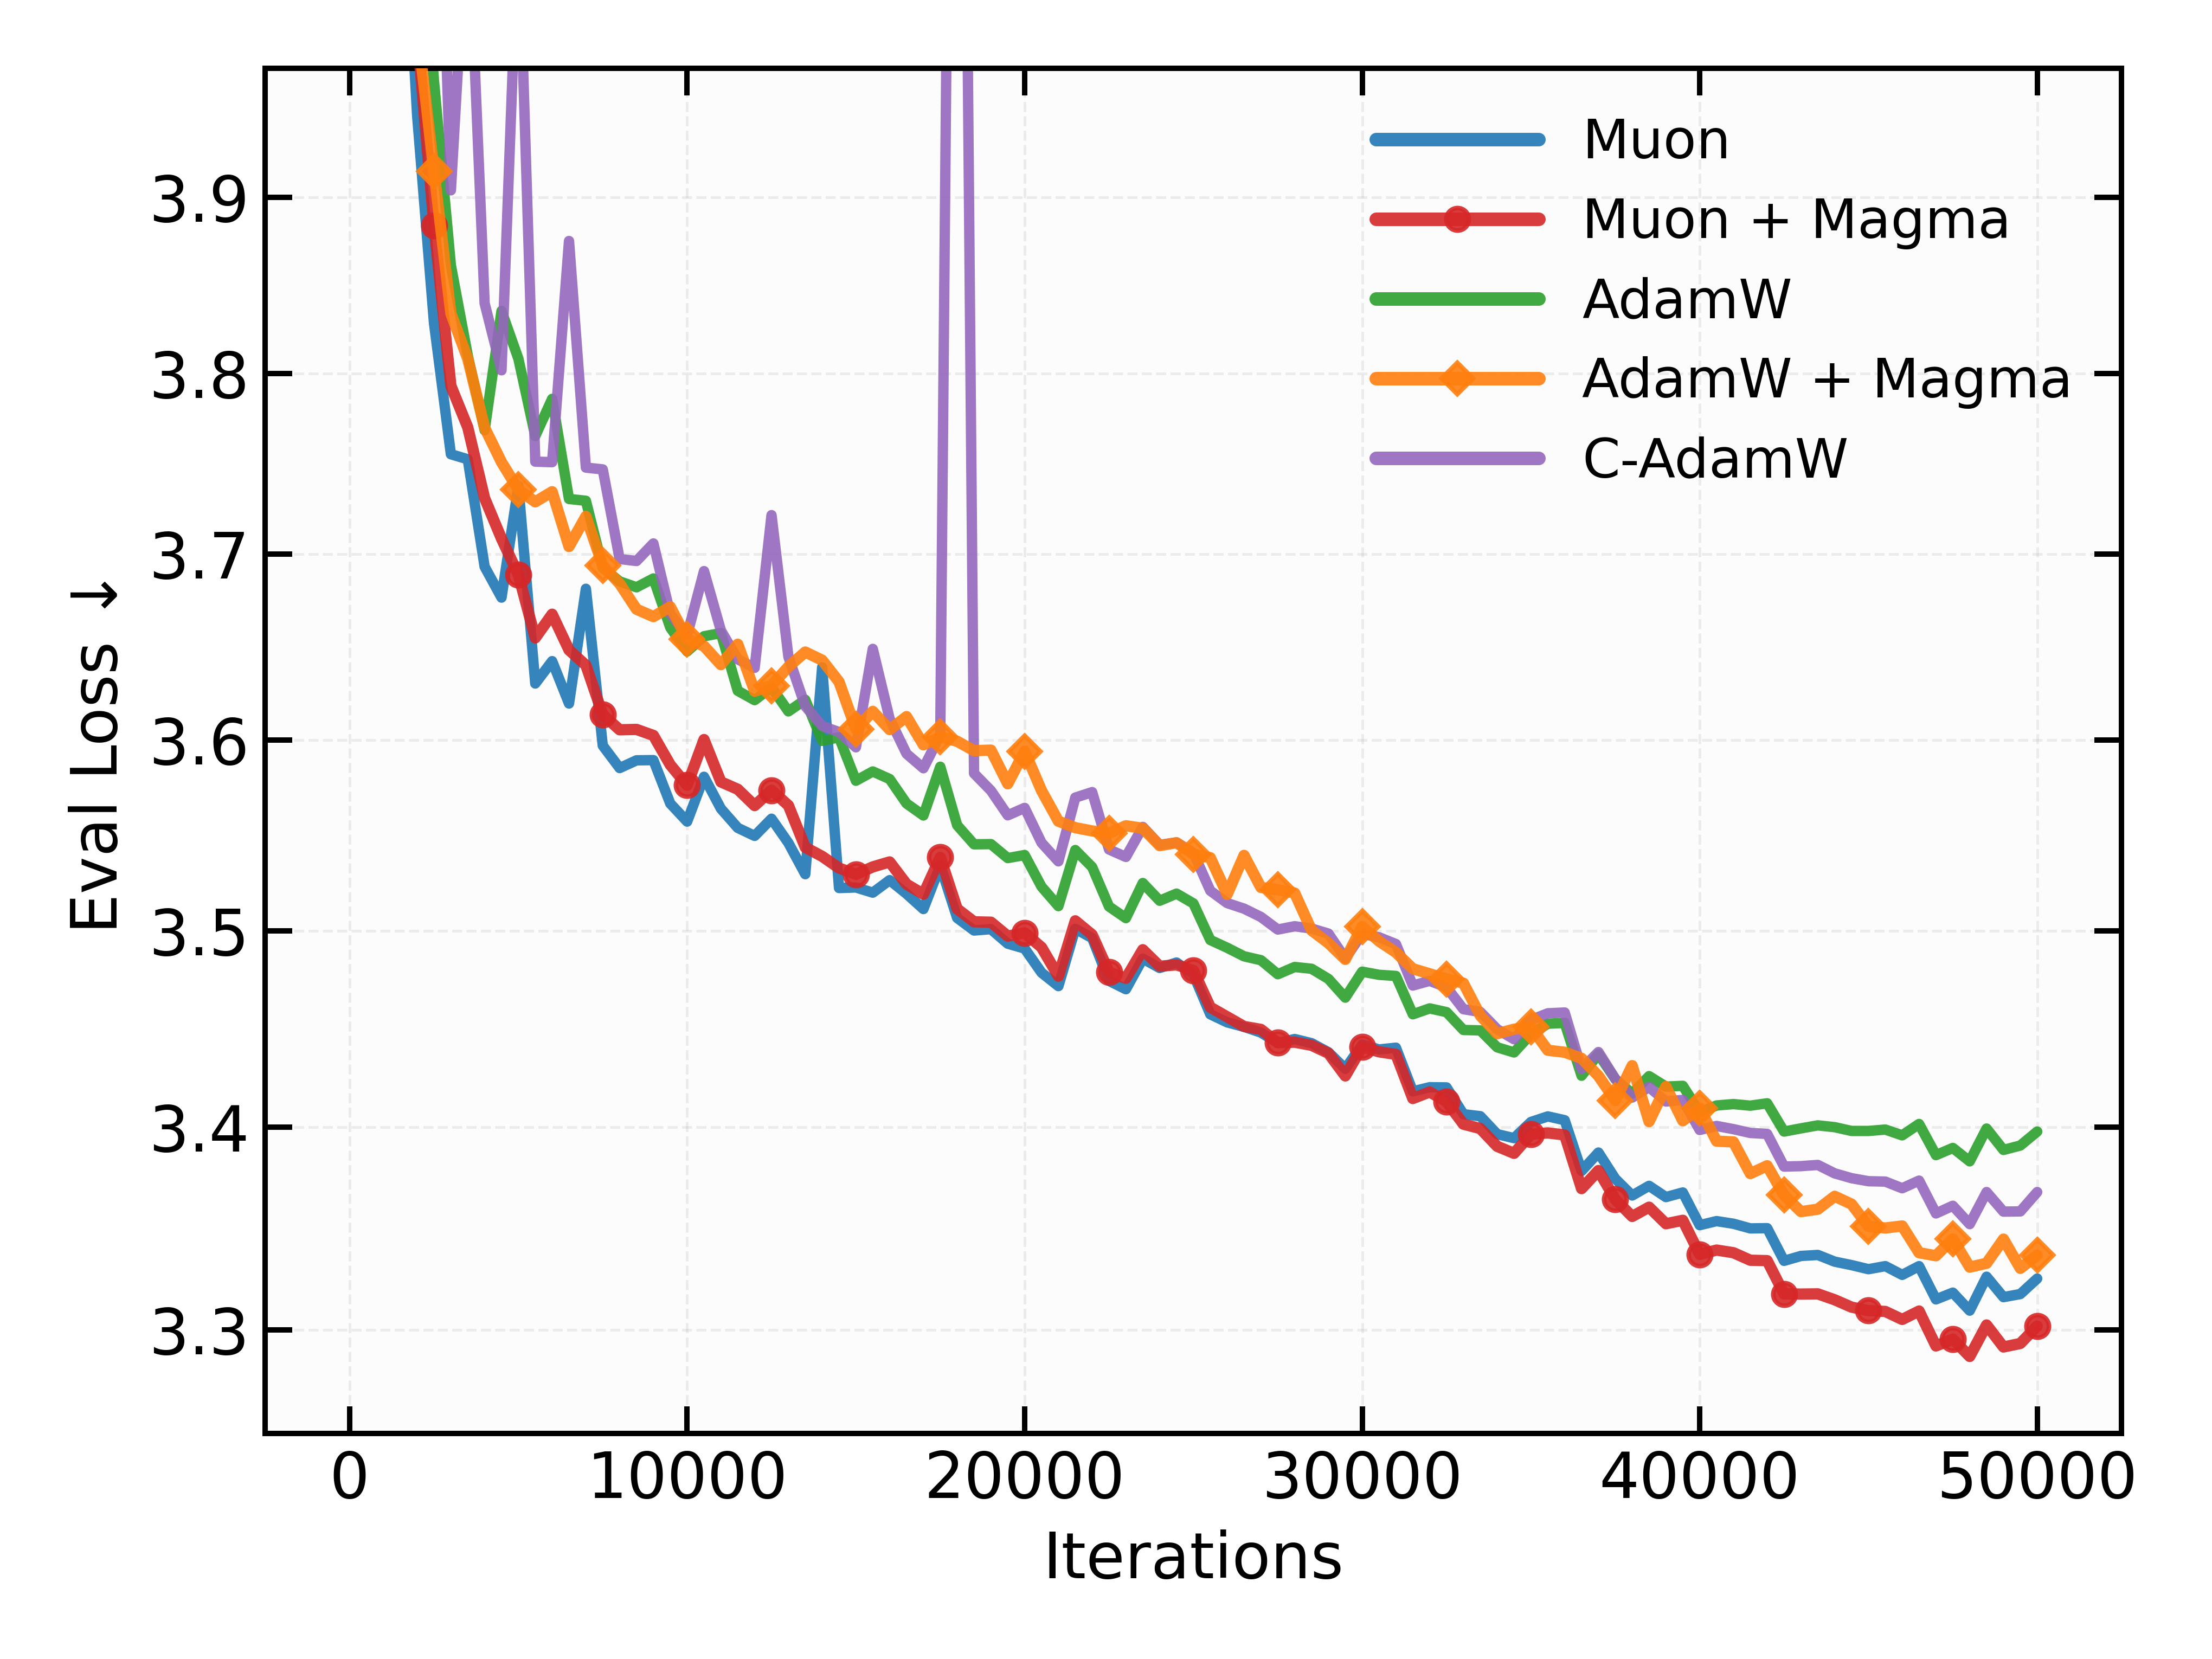
\includegraphics[width=0.49\textwidth]{figs/nanomoe_new.png}
\end{center}
\vskip -0.15in
\caption{OpenWebText 上预训练 Nano MoE 模型的优化轨迹。} 
\label{fig:nano-moe}
\vskip -0.15in
\end{figure}


图 \ref{fig:nano-moe} 的结果表明，在 MoE 场景中，Magma 能稳定提升 Adam 与 Muon 的性能。作用于 Adam 时，Magma 在训练中段收敛较慢，但最终性能更优。与 Llama 预训练一致，Magma 也显著优于同样利用动量-梯度对齐的 Cautious Optimizer（C-Adam），从而进一步验证了 Magma 通过结构化随机掩码实现几何正则化的有效性（\S \ref{sec:mainsection}）。


值得注意的是，当与 Muon 结合时，Magma 取得了整体最佳性能，显著优于全部基线。 
这表明，Magma 基于随机掩码的更新调制与结构化预条件主要作用于优化过程的不同维度，能够以互补方式共同塑造训练动力学与收敛几何。考虑到现代 MoE-LLM 训练越来越依赖 Muon \citep{jordan2024muon}、SOAP \citep{vyas2024soap} 等复杂预条件器，这些结果凸显了 Magma 作为一种稳健且高效增强方案，可无缝集成进大规模优化流水线。




\begin{figure}
% \vskip -0.1in
\begin{center}
% 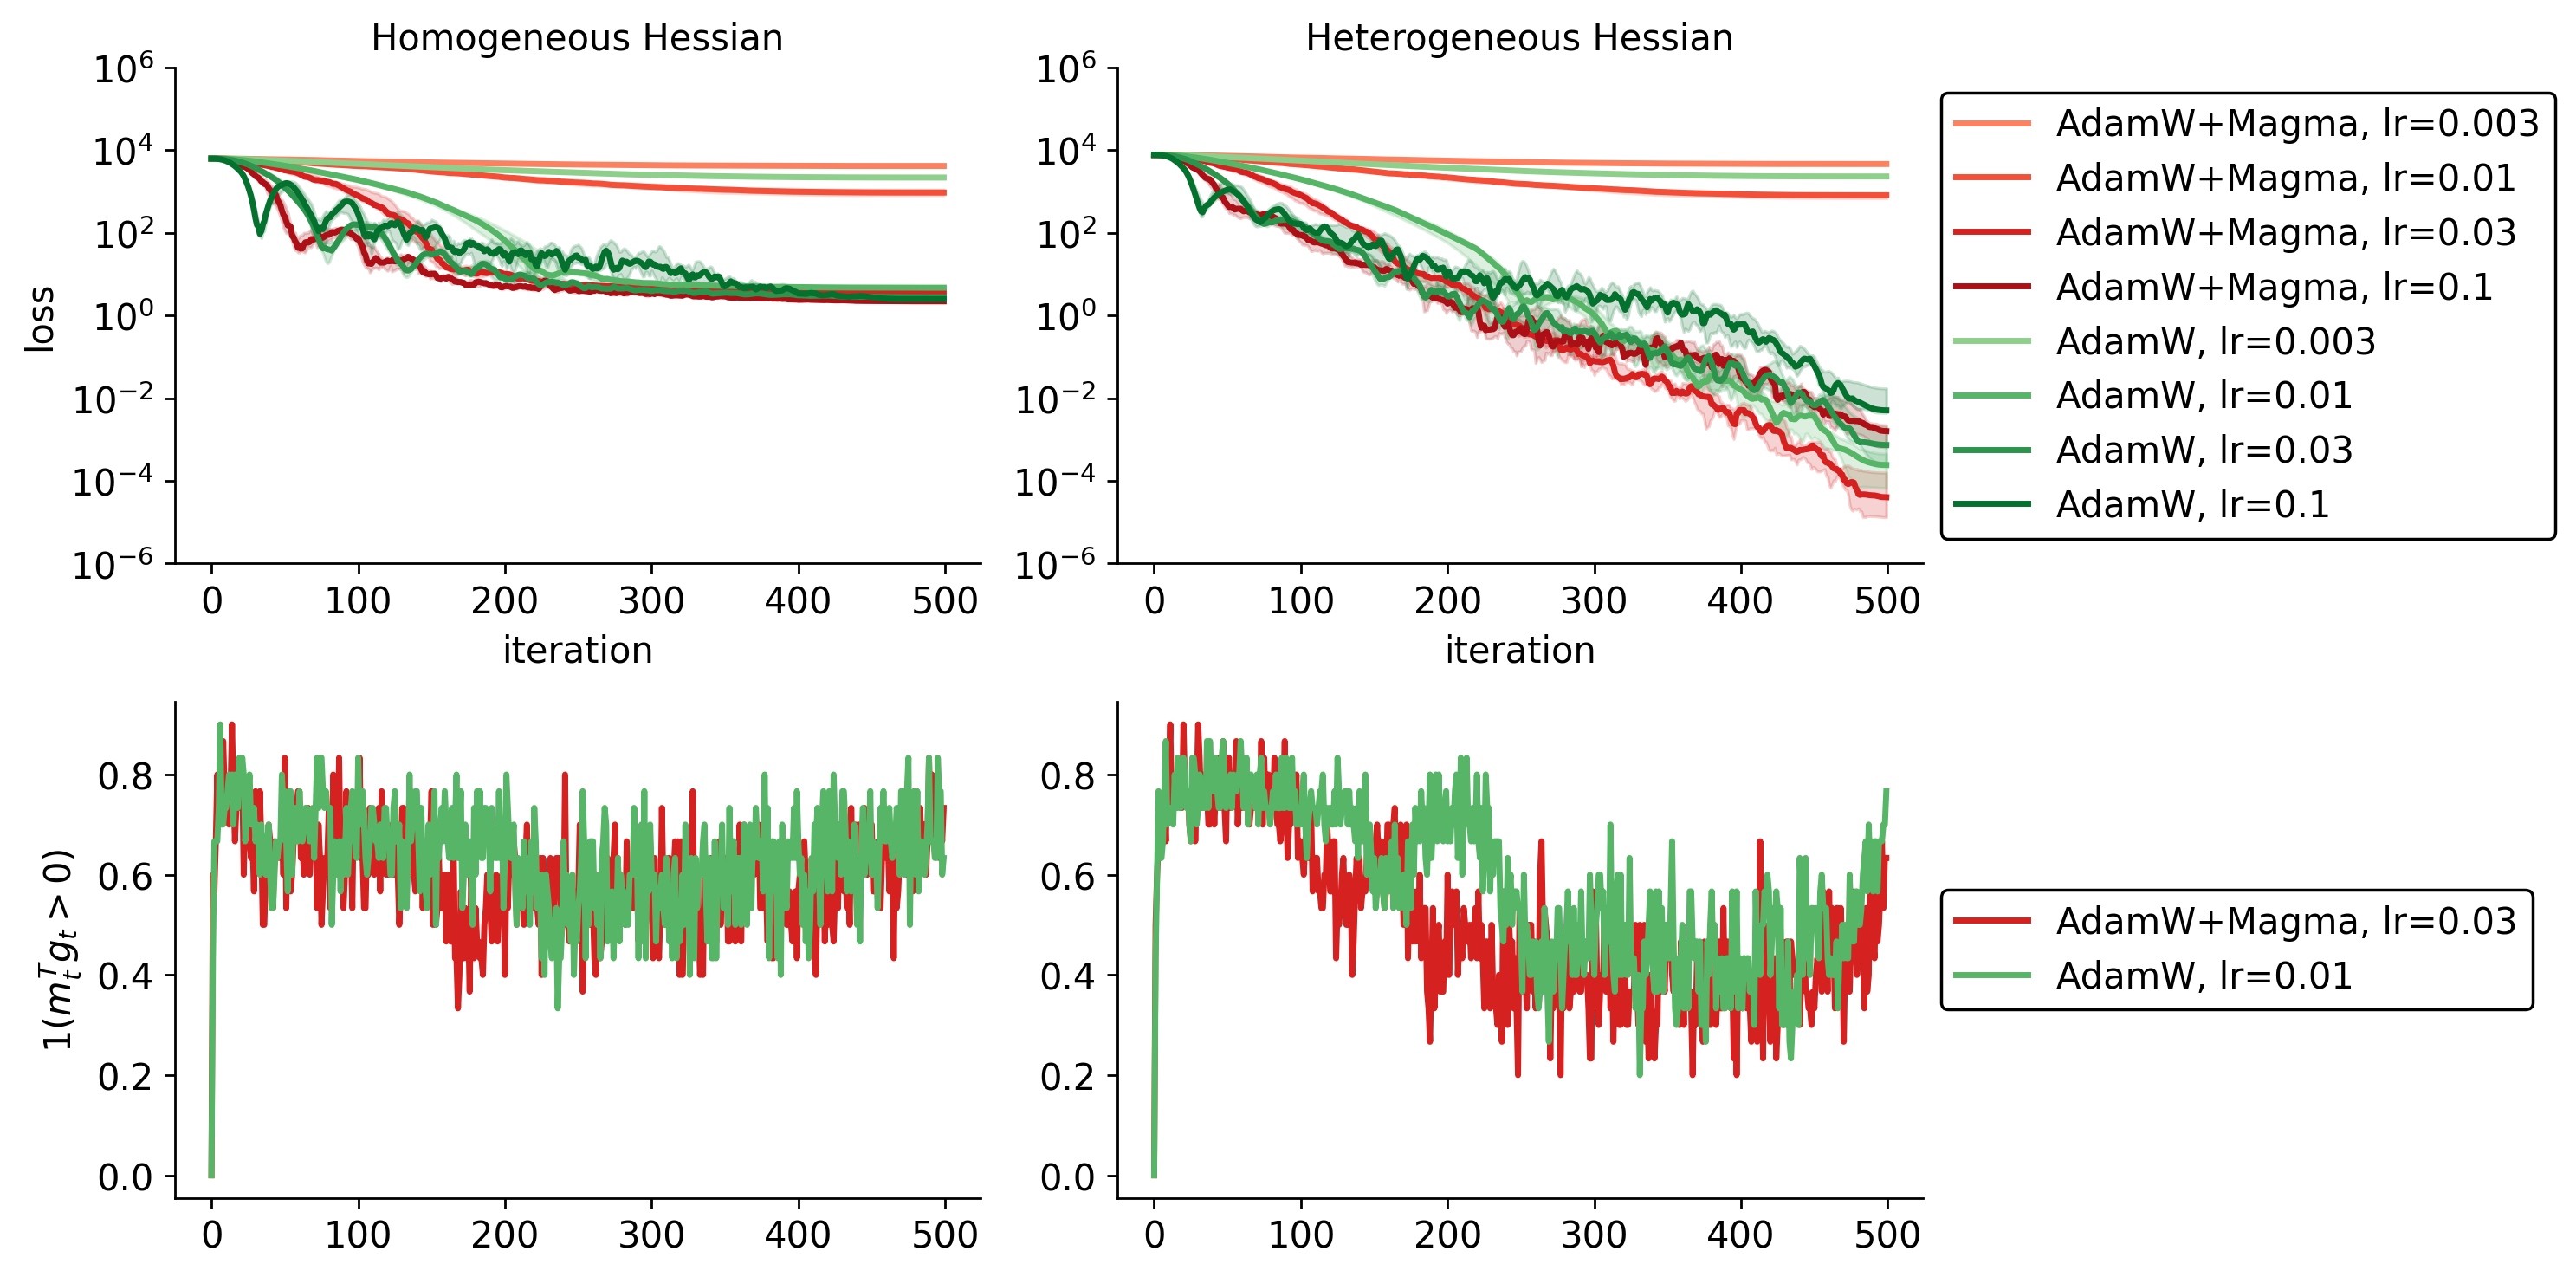
\includegraphics[width=0.95\textwidth]{figs/h.png}
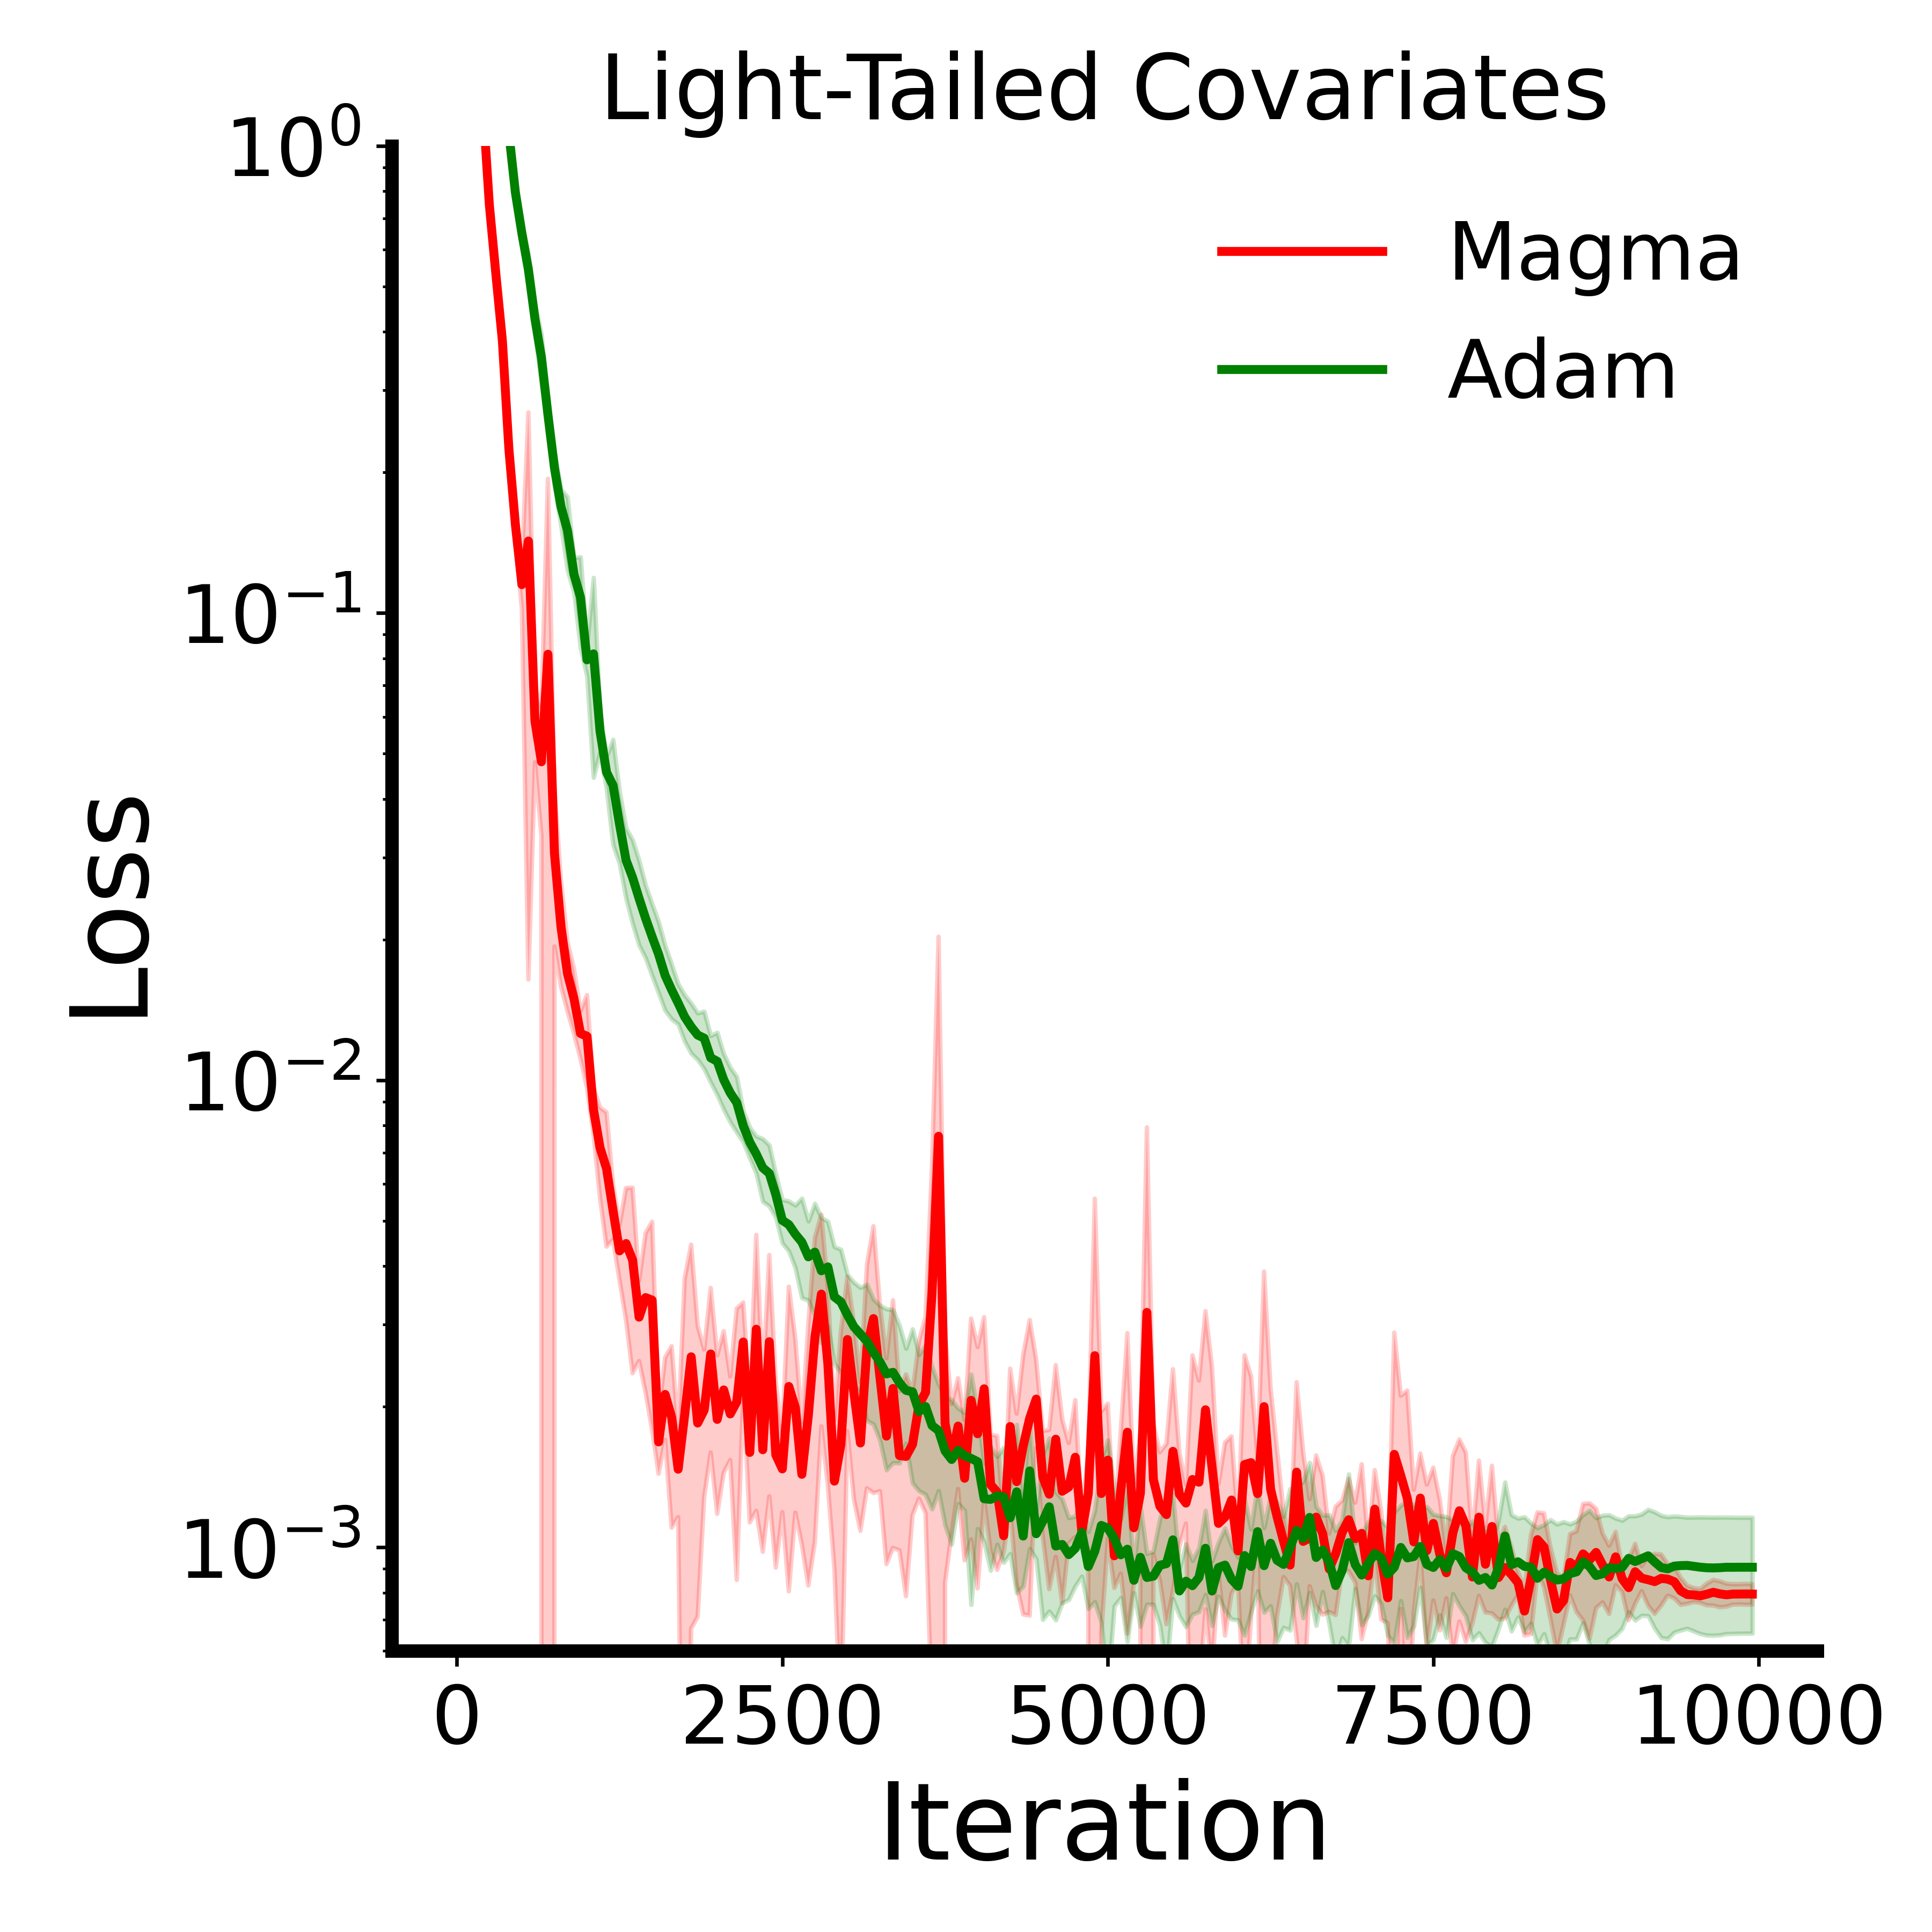
\includegraphics[width=0.235\textwidth]{figs/loss_layer3_N20_normal-lt.png}
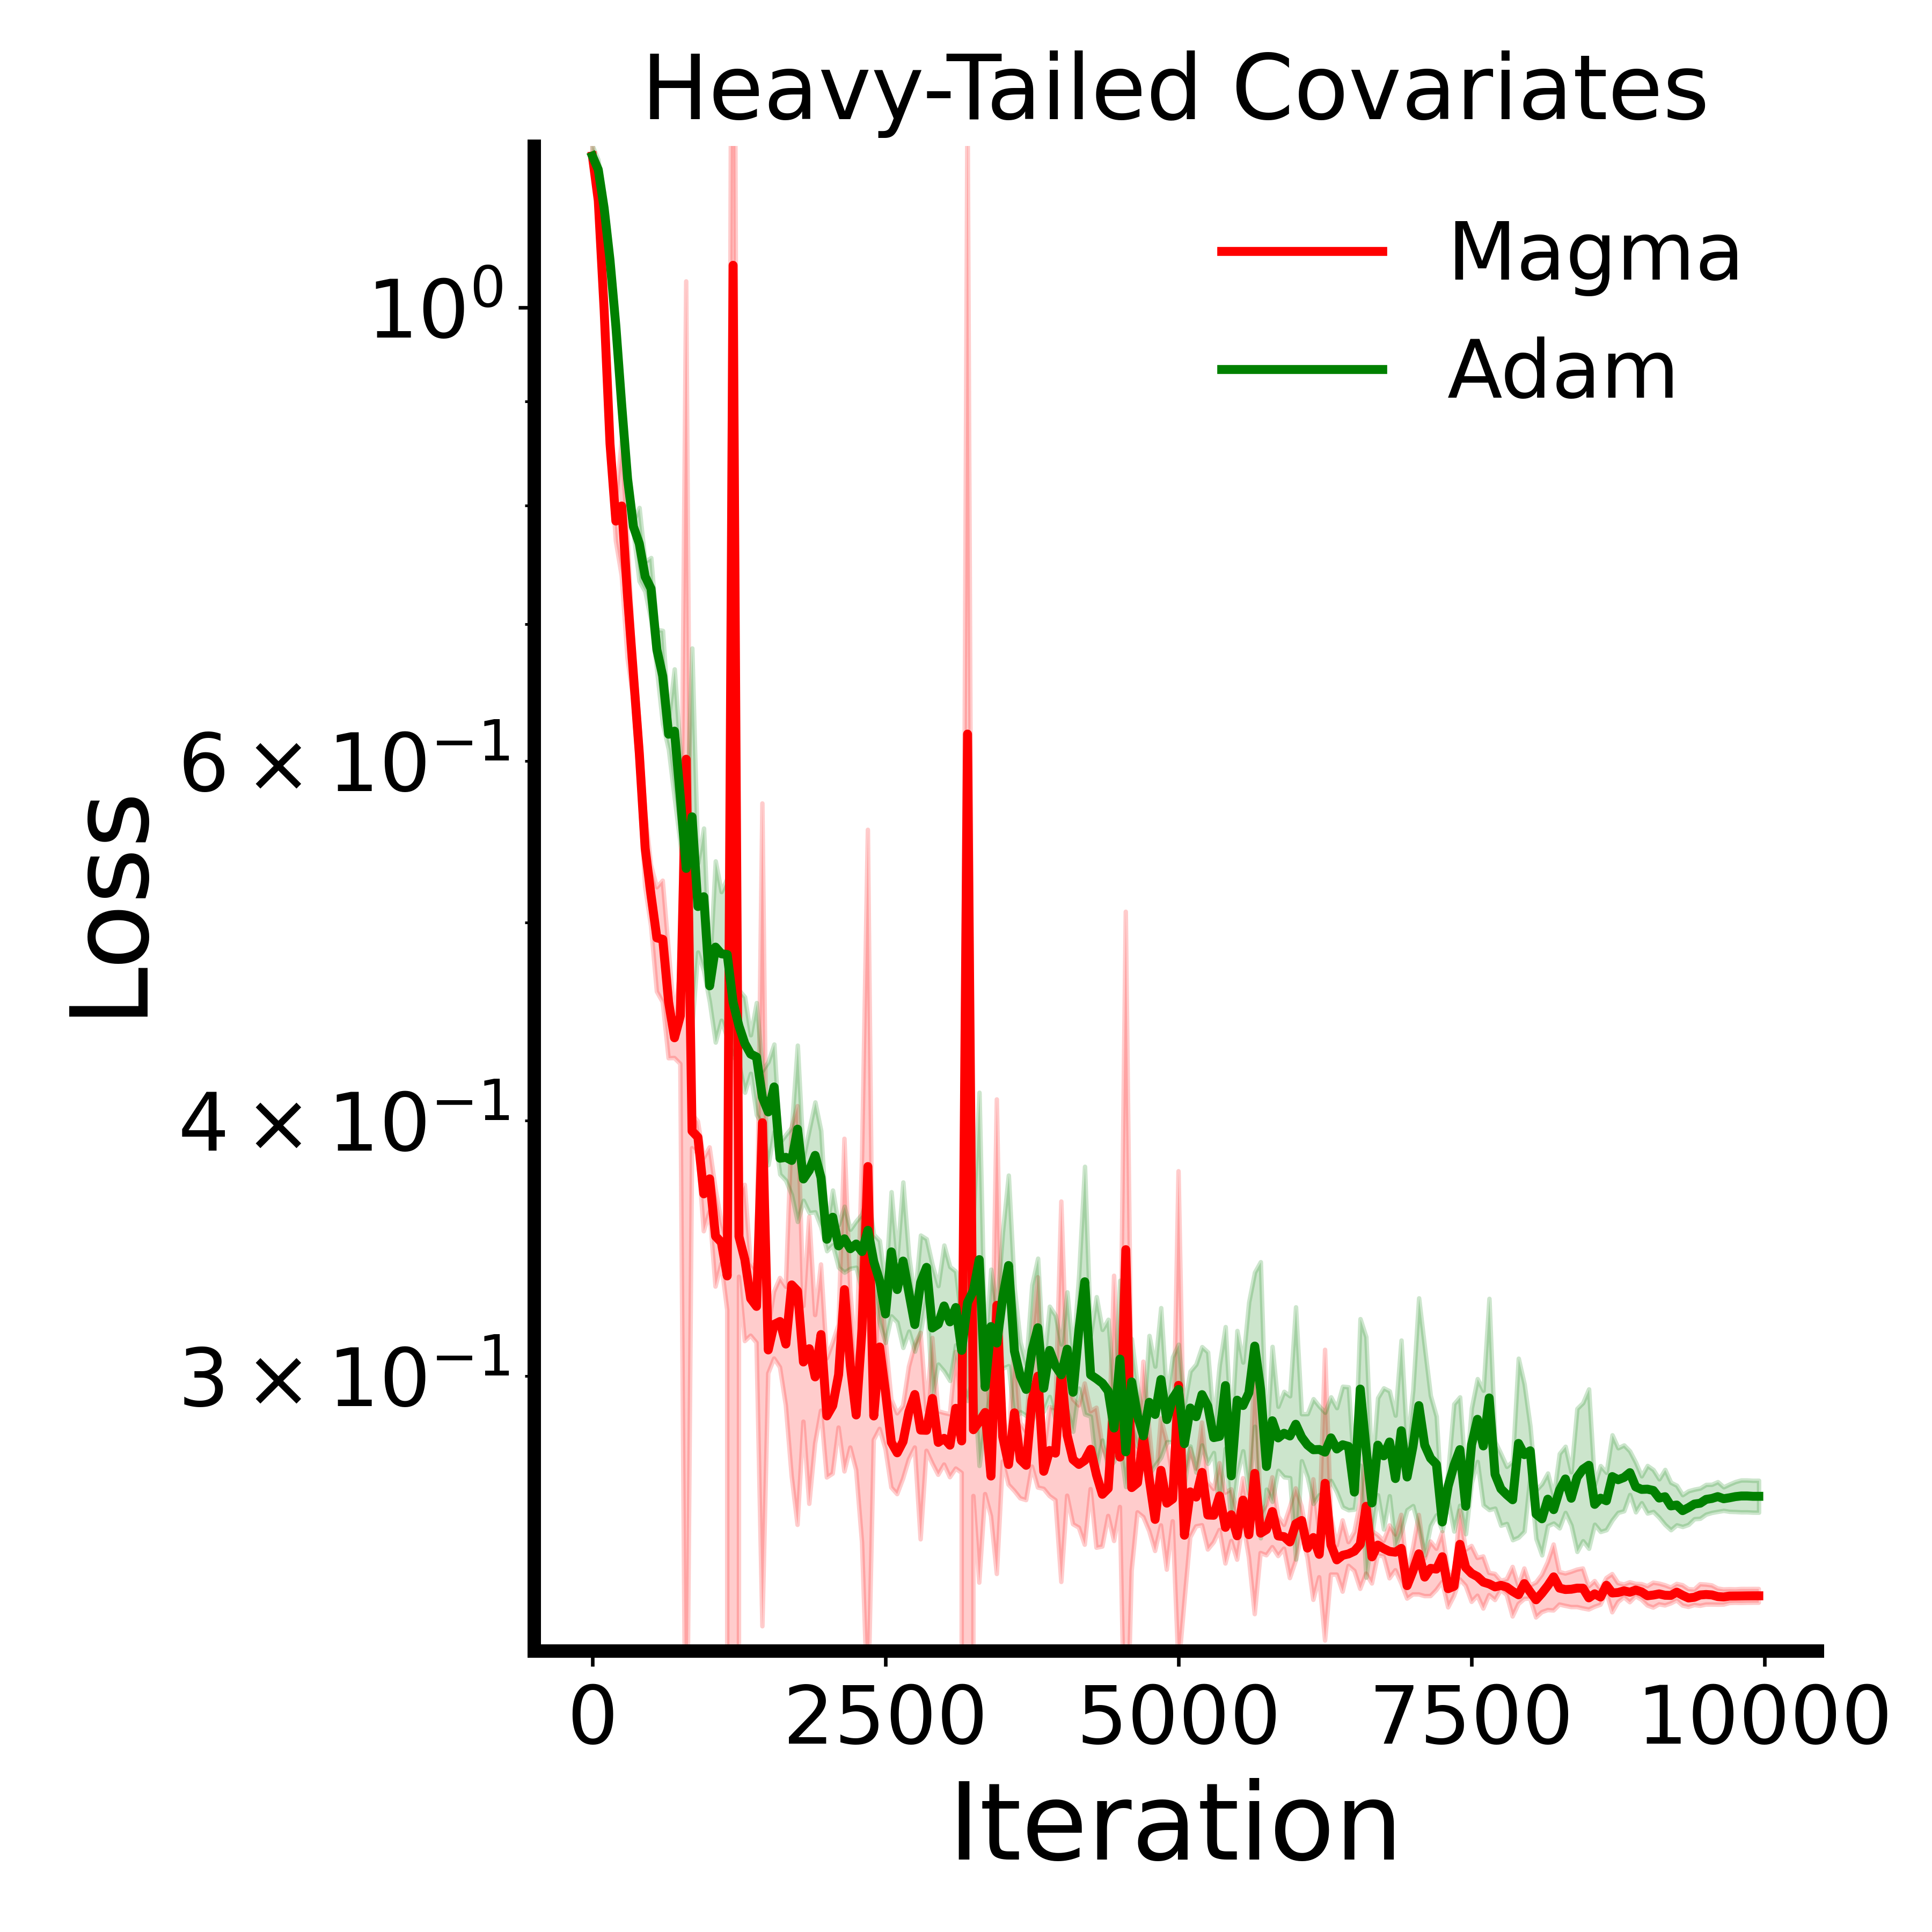
\includegraphics[width=0.235\textwidth]{figs/loss_layer3_N20_gamma-ht.png}
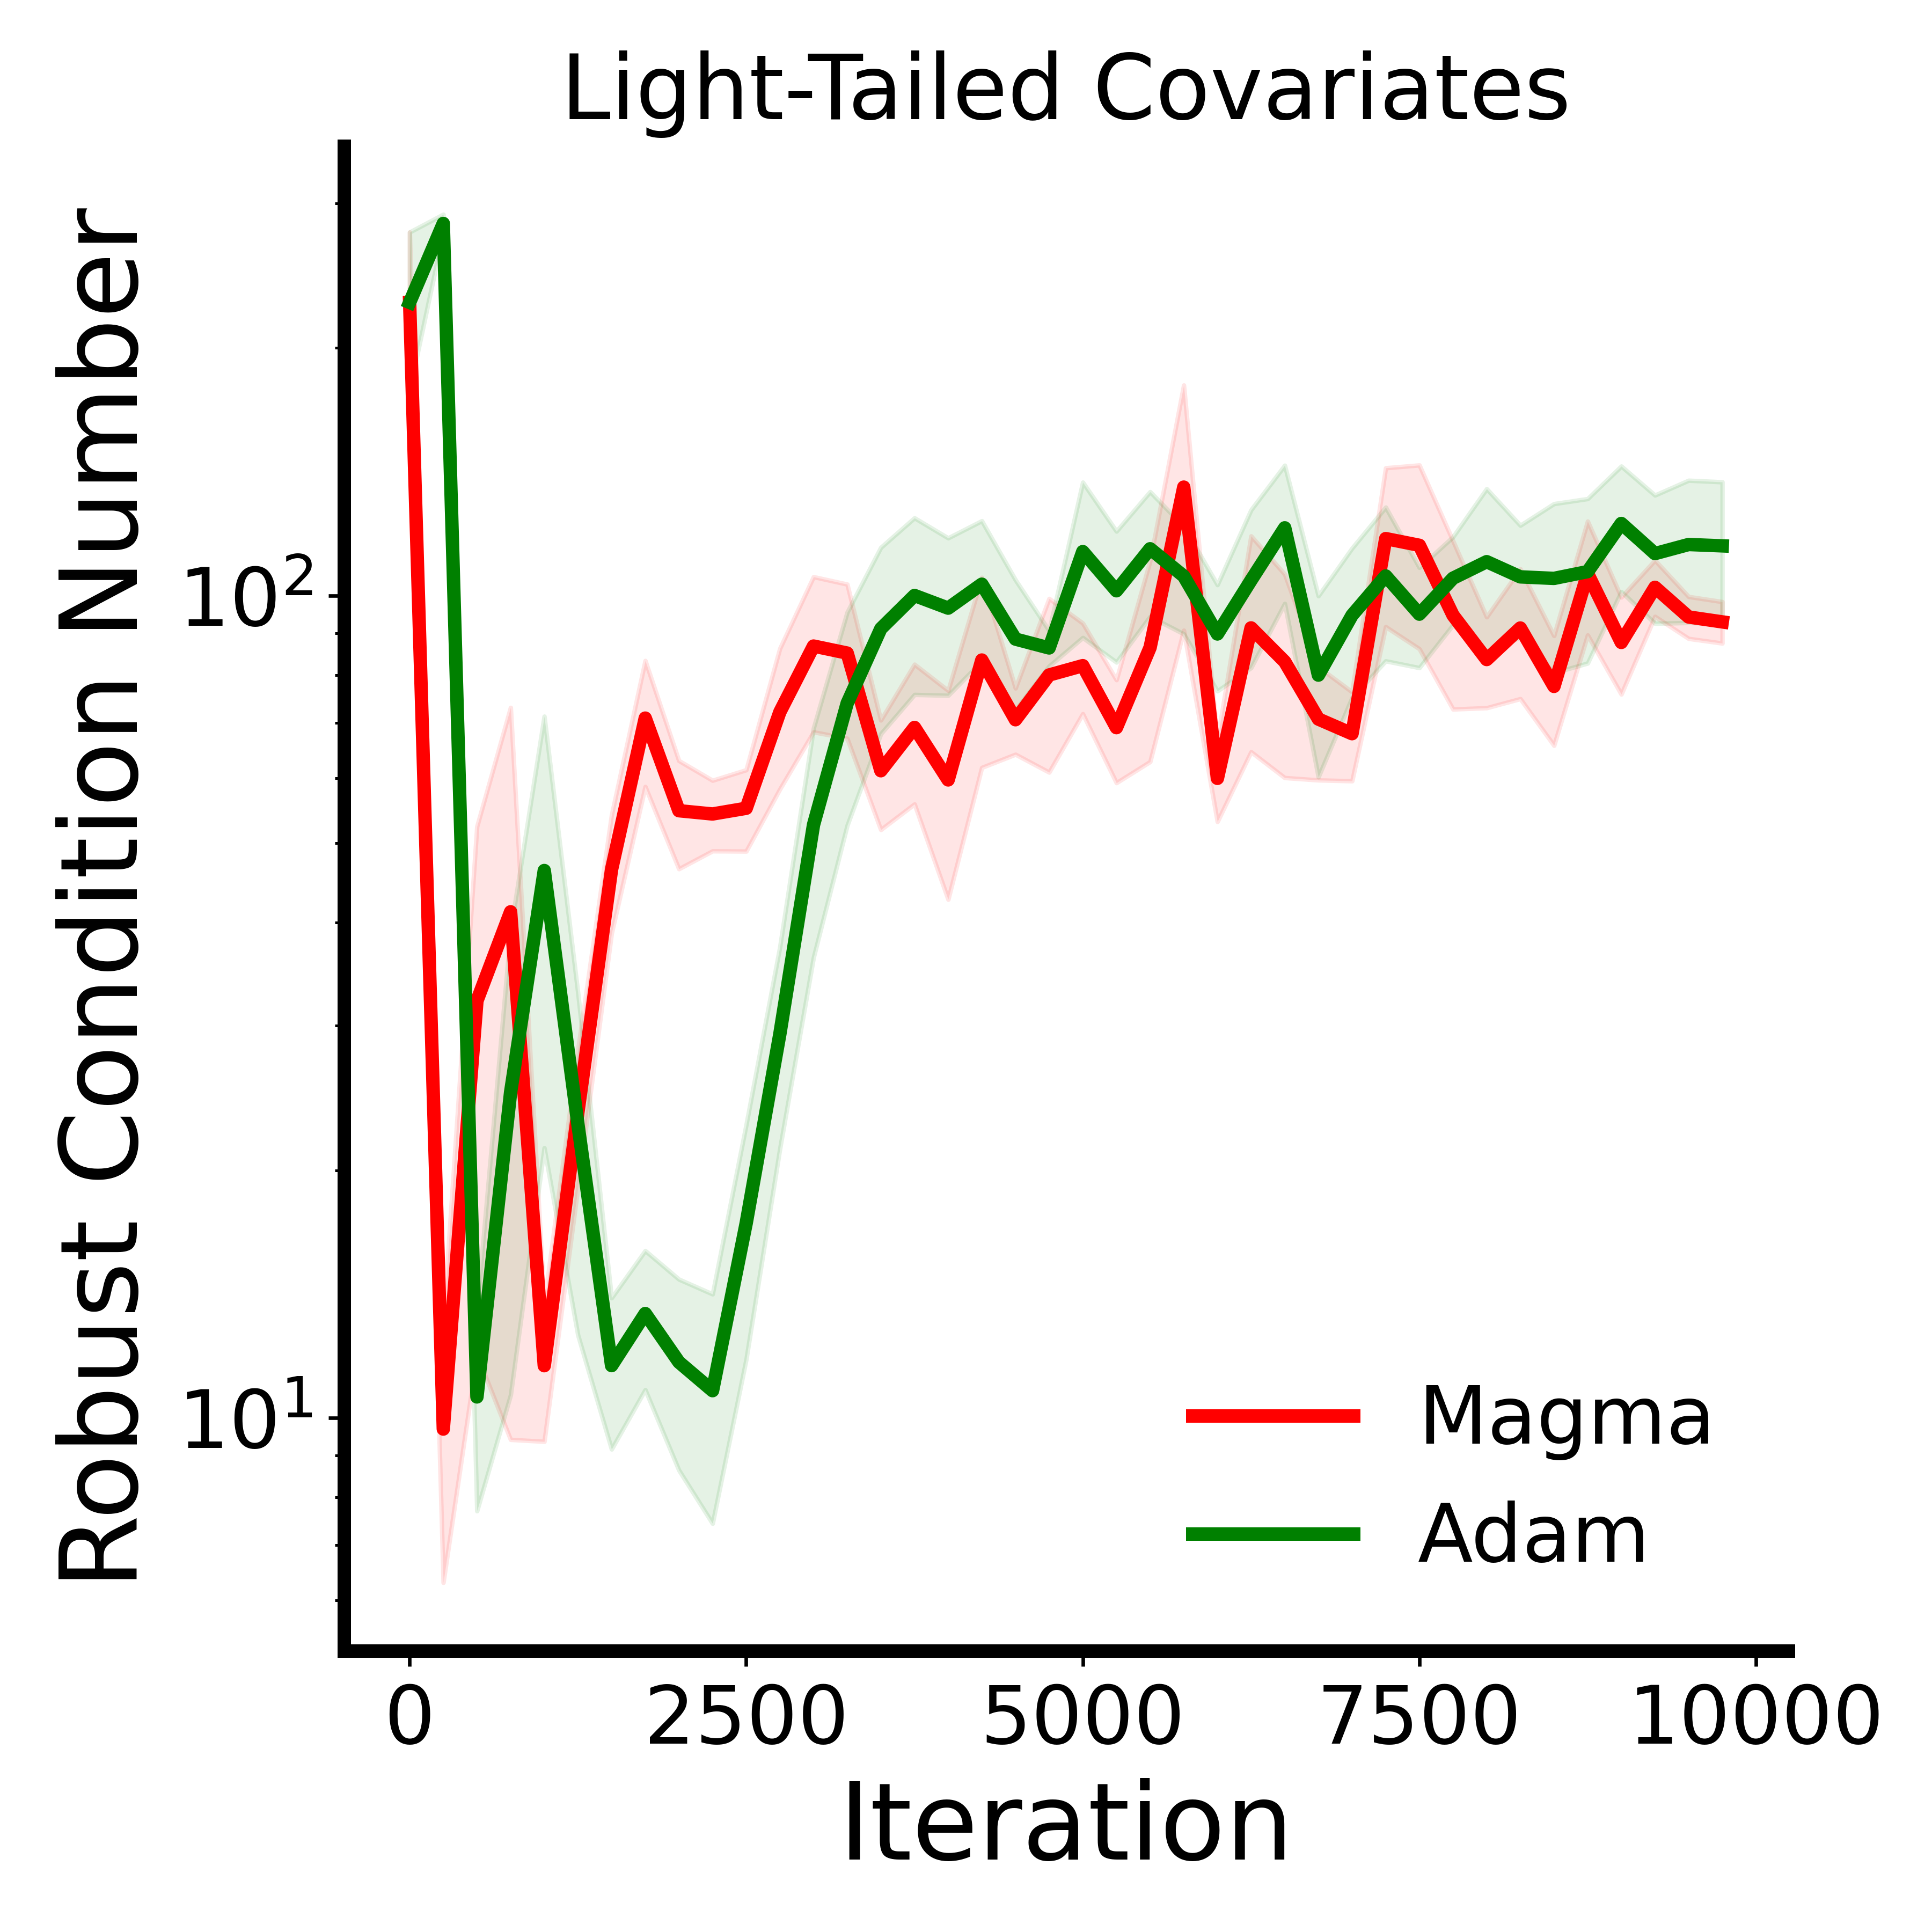
\includegraphics[width=0.235\textwidth]{figs/condition_number_layer3_N20_normal-lt.png}
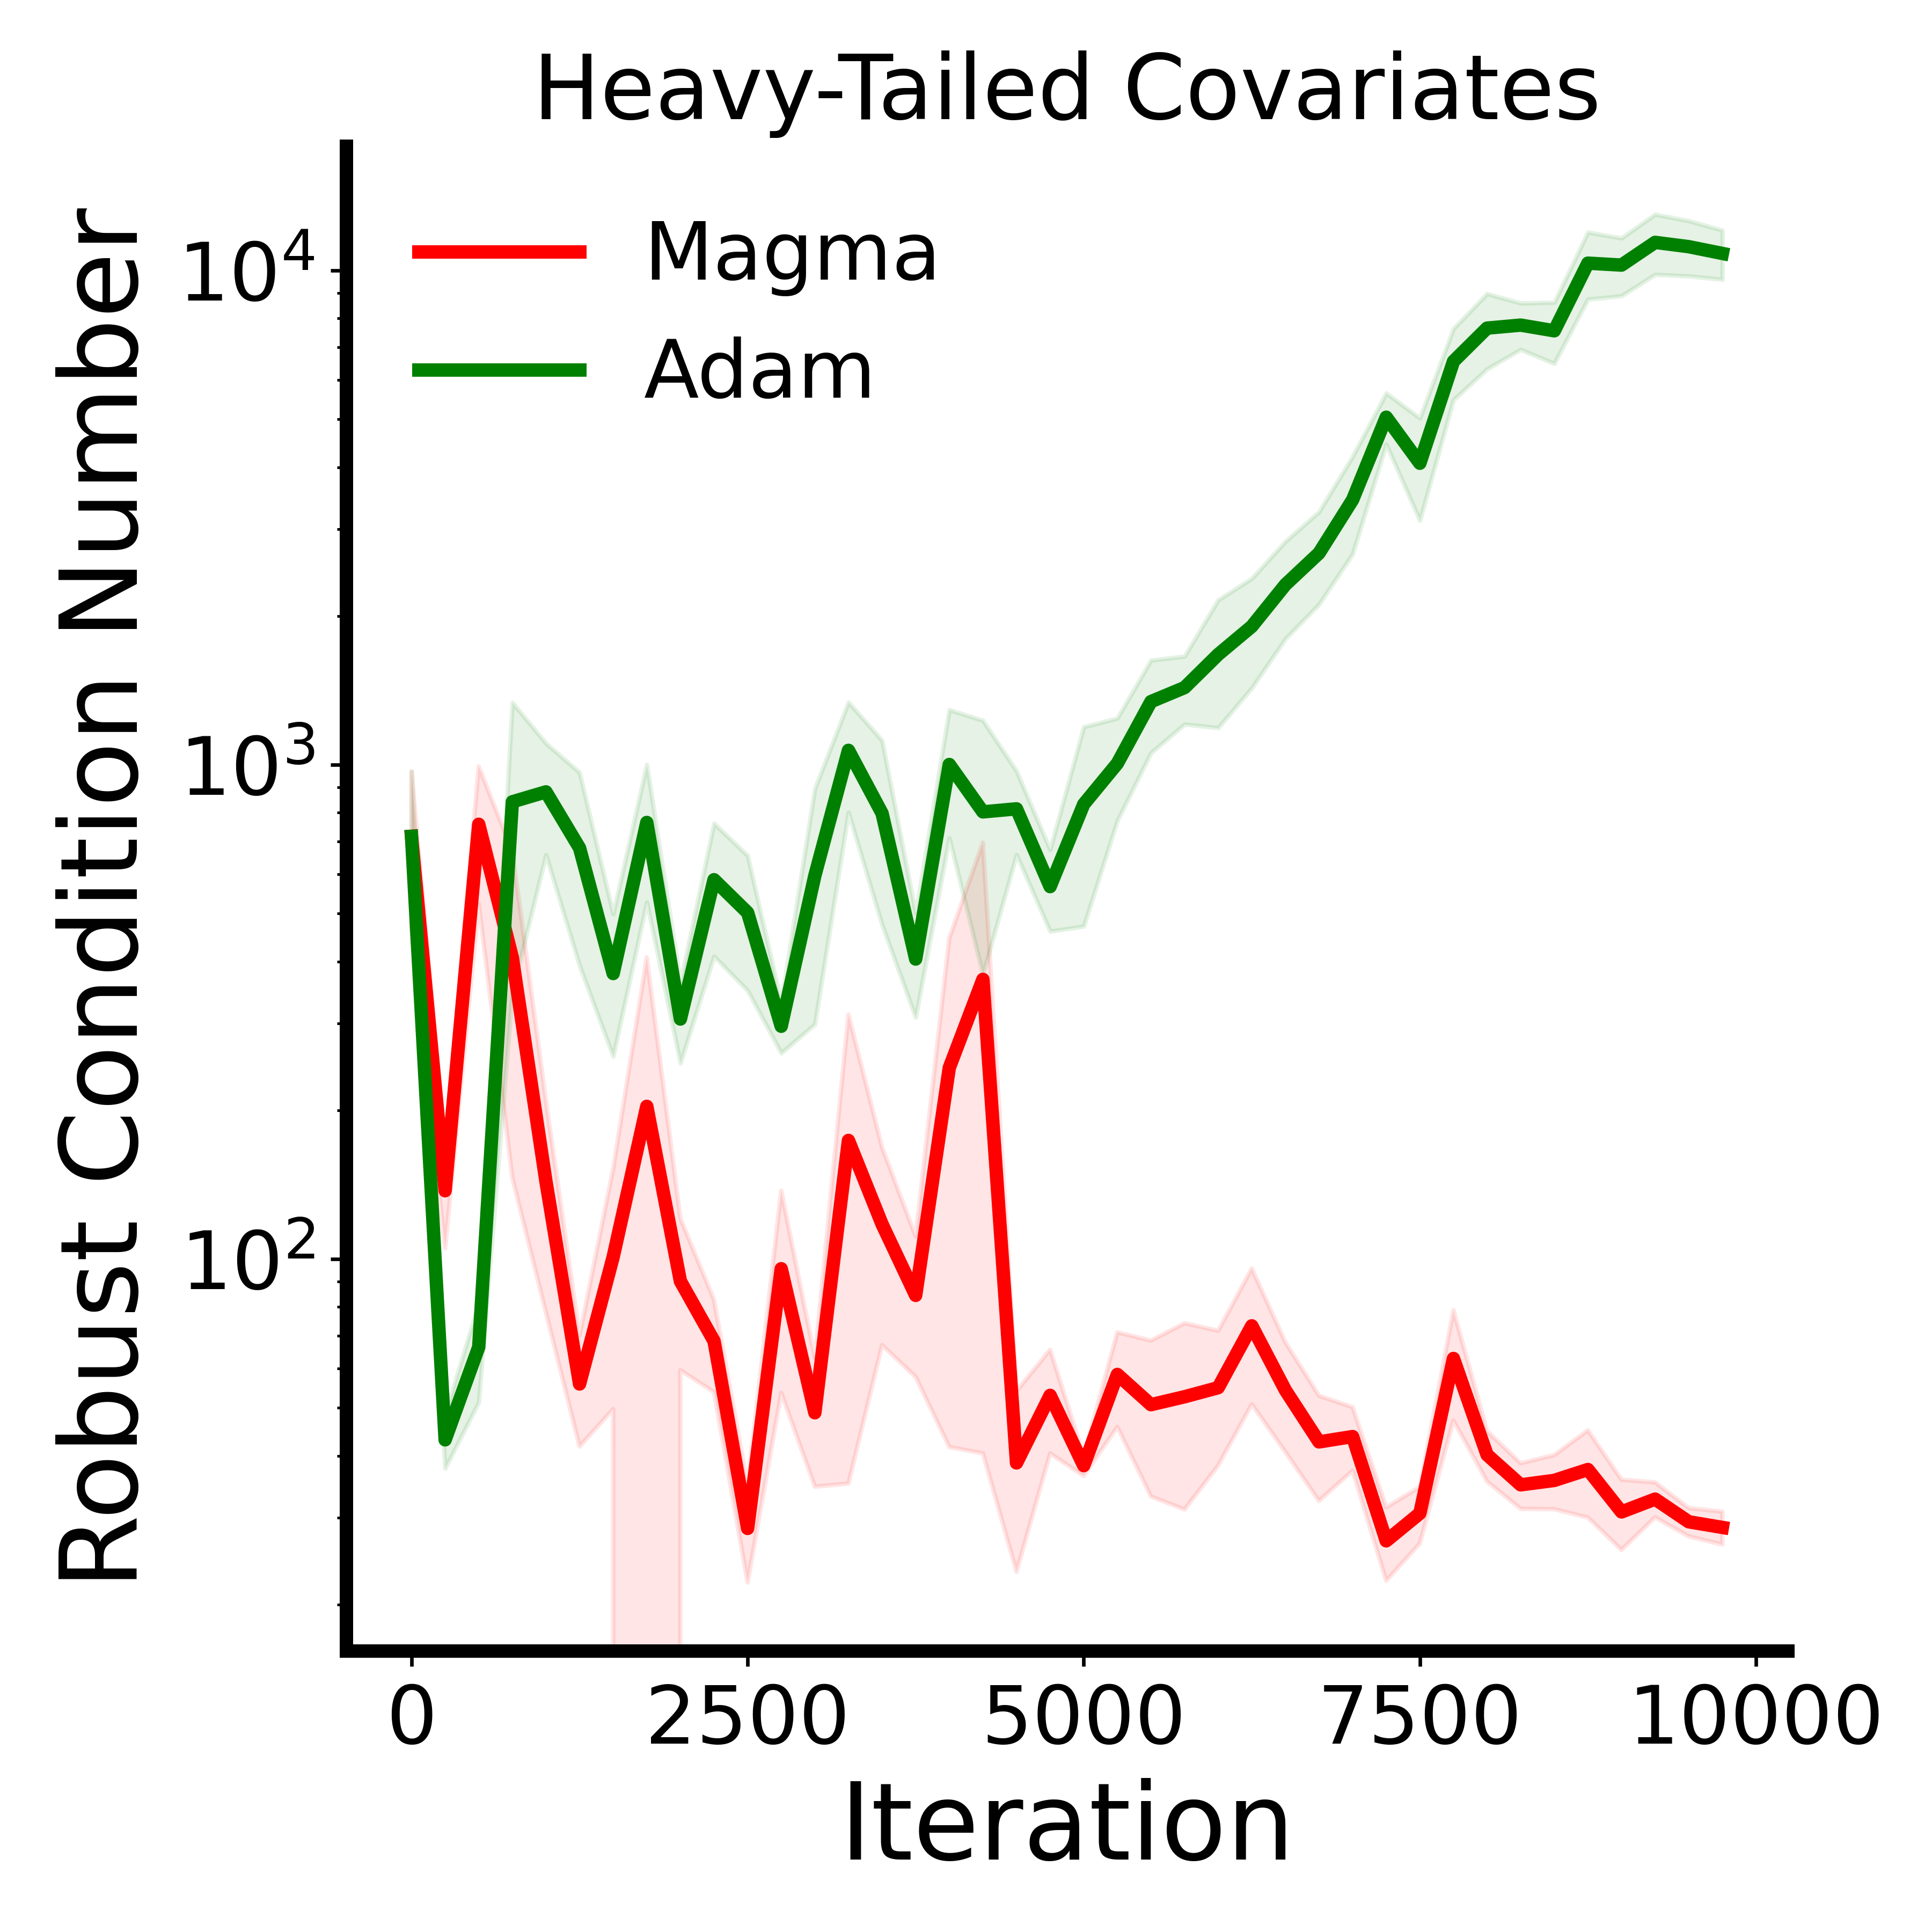
\includegraphics[width=0.235\textwidth]{figs/condition_number_layer3_N20_gamma-ht.png}
\end{center}
\vskip -0.1in
\caption{\textit{Magma 在轻尾与重尾数据分布下的表现。} 
\underline{\textbf{\emph{上：}}} Adam 与 Magma 的优化轨迹。 
\underline{\textbf{\emph{下：}}} 鲁棒条件数，定义为损失 Hessian 最大特征值与中位特征值之比。  
}
\label{fig:heavy-tailed}
\vskip -0.1in
\end{figure}




\begin{figure*}
\vskip -0.06in
\begin{center}
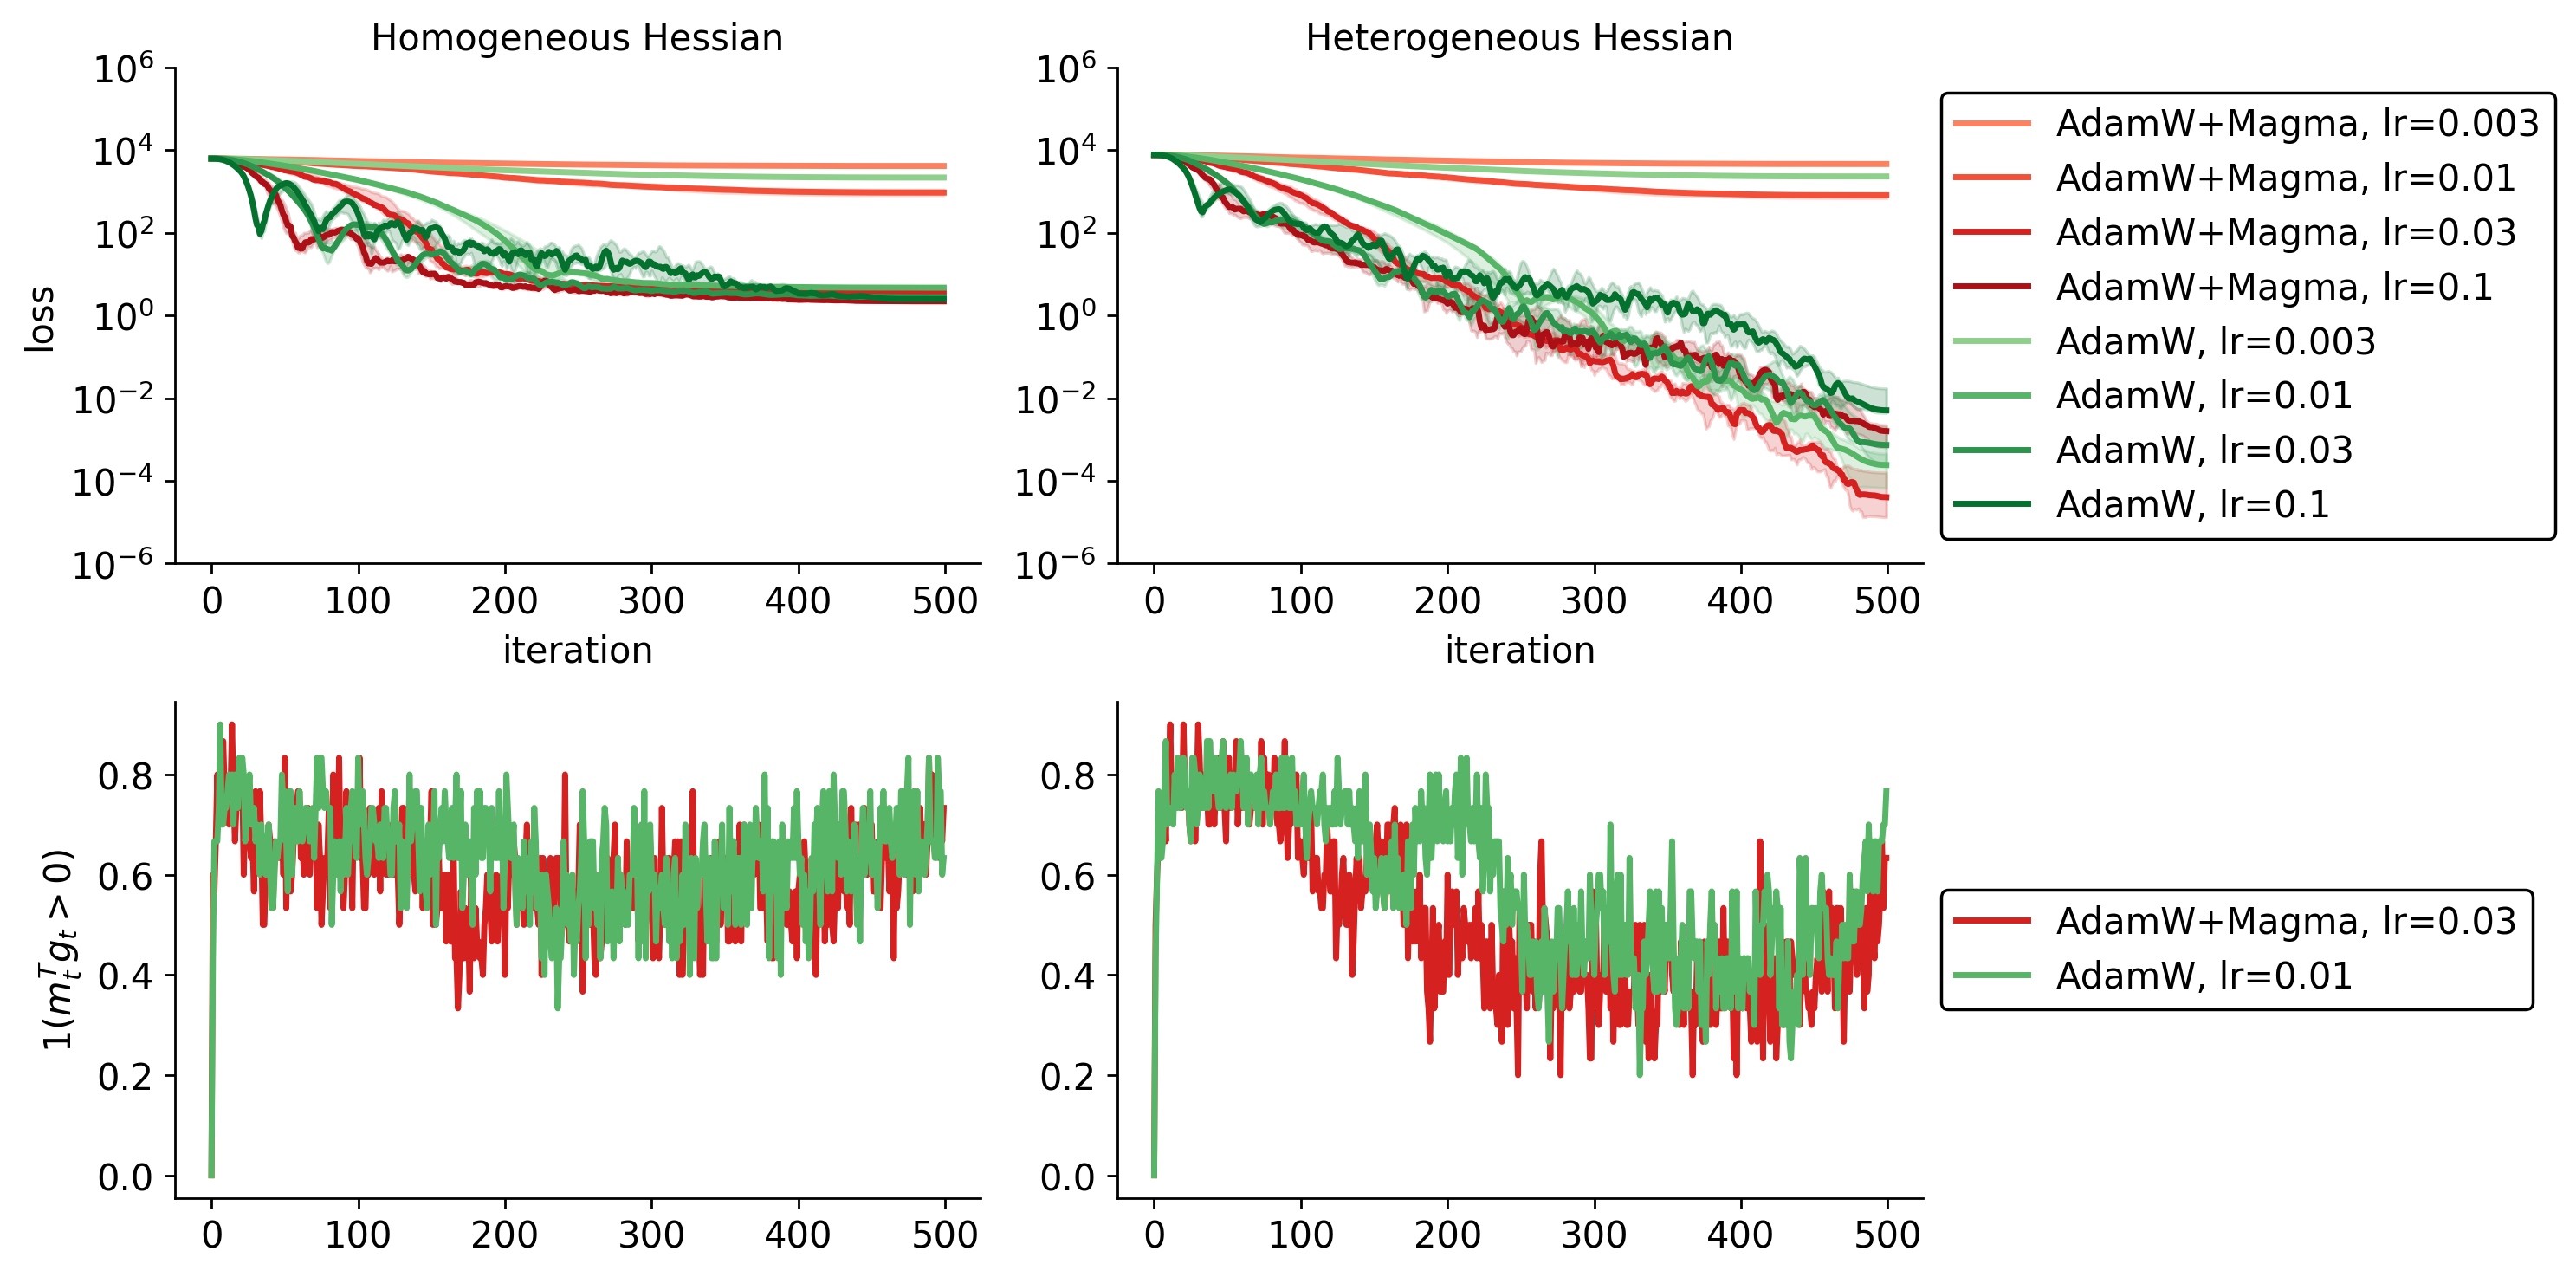
\includegraphics[width=0.98\textwidth]{figs/h.png}
\end{center}
\caption{\textit{Magma 在同质与异质二次问题上的表现。} 
\underline{\textbf{\emph{上：}}} 在具有相同特征谱但不同块结构的二次目标上，AdamW 与 Magma 的优化轨迹。 
\underline{\textbf{\emph{下：}}} 每个块的平均梯度-动量对齐度。 
}
\label{fig:quadratic}
\vskip -0.1in
\end{figure*}




\subsection{重尾梯度噪声下的 Magma}
自回归语言模型训练的一个显著特征是存在重尾随机梯度噪声 \citep{zhang2019gradient, kunstner2024heavy}。 
为隔离并研究重尾噪声对优化动力学的影响，我们采用 \citet{ahn2023linear} 提出的可控基准评估 Magma。该基准在抽象 Transformer 训练的同时，能忠实复现实践中的关键经验现象，包括 LLM 预训练中 Adam 与 SGD 的性能差距。
该基准考虑以元学习形式训练简化线性 Transformer 来求解随机线性回归任务 \citep{garg2022can,von2023transformers,akyurek2022learning}。 
在该基准中，我们考察两种数据机制：\textit{轻尾}与\textit{重尾}。在重尾设置下，我们修改输入采样分布以增强协变量尾部行为，从而在优化过程中诱导重尾随机梯度噪声。完整实验细节见附录 \ref{appx:ahn_linear_benchmark}。




图 \ref{fig:heavy-tailed}（上）比较了在正态协变量与重尾协变量下 Adam 与 Magma 的优化轨迹。 
在正态噪声下两者表现相近；而在重尾设置下，Magma 显著优于 Adam，这有助于解释其在 LLM 预训练中的强经验表现——在该场景中重尾数据普遍存在 \citep{kunstner2024heavy,ahn2023linear}。 
鉴于 Adam 已知对重尾分布具有鲁棒性，这一结果尤为值得关注。


为进一步分析该行为，图 \ref{fig:heavy-tailed}（下）报告了训练轨迹上的鲁棒条件数 \citep{jiang2023does}。在重尾噪声下，Magma 持续达到显著更小的条件数，表明其更新更受限于损失景观中条件更良好的区域。这体现了缩放随机掩码所诱导的依赖曲率几何正则化：它会有选择地抑制由曲率与噪声主导的方向，从而提升对极端梯度波动的鲁棒性。



\subsection{异质二次问题上的 Magma}
为进一步验证 Magma 在异质景观中的有效性，我们在近期工作采用的可控二次基准上评估 Magma \citep{zhang2024transformers, orvieto2025search}。
该基准包含两个\emph{特征谱完全一致}但块级曲率结构不同的二次目标。两者损失形式均为 $l(\vw) = \tfrac{1}{2} \vw^\top \mH \vw,$ 其中 $\mH$ 的特征值跨越三个数量级。关键差异在于特征值排列方式：在\emph{同质}设置中，相同尺度特征值在块内分组；而在\emph{异质}设置中，每个块混合了量级差异极大的特征值，导致强曲率失配。 
尽管该结构简单，但它在定性上更贴近自回归 Transformer 的损失几何，而不同于 CNN 常见的更强尺度分离曲率。完整细节见附录 \ref{appx:hetero_quad_setup}。



图~\ref{fig:quadratic}（上）给出了两种 Hessian 结构下的优化轨迹。
在同质问题上，Magma 与 AdamW 表现相当，Magma 在早期阶段略快收敛。  
然而在异质问题上，尽管已有结论表明 AdamW 显著优于 SGD 等非自适应方法 \citep{zhang2024transformers,orvieto2025search}，Magma 仍实现了更快收敛与更低最终损失。  
这与预训练实验中的增益一致（见表 \ref{table:benchmark_c4}），表明 Magma 在曲率既病态又跨参数子空间失配的场景中特别有效。

重要的是，这一优势并不扩展到曲率更接近同质情形的架构。 
例如，在 CIFAR-10 分类任务上应用于 ResNet-50 时，Magma 相较 AdamW 并无提升（经过精调配置训练 100 轮后测试精度为 94.46\% vs.\ 93.82\%），这进一步支持其收益与 Transformer 式损失几何相关的假设。


图~\ref{fig:quadratic}（下）分析了 AdamW 与 Magma 在每个块内的平均梯度-动量对齐度。  
与预期一致，同质 Hessian 在所有块上都表现出更高对齐度，反映其更温和的条件数特性。
值得注意的是，尽管 Magma 显式抑制与累积动量冲突的更新，它并未显著提高对齐分数本身。
这表明 Magma 的收益并非源于改变动量统计量，而是来自强化瞬时梯度与长期下降方向之间的一致性。



% % ========================================================================
% % ========================================================================
% % ========================================================================
% %         讨论
% % ========================================================================
% % ========================================================================
% % ========================================================================
\section{讨论} \label{sec:convergence_analysis}
我们从经典优化理论视角分析 Magma 中缩放随机掩码的作用。 

\textbf{设定。}
考虑 $\theta \in \R^d$，可分解为 $\theta = (\theta^{(1)}, \theta^{(2)}, \cdots, \theta^{(B)})$，其中 $\theta^{(b)} \in \R^{d'}$ 且 $B d' = d$。我们假设目标函数下界存在：$l_* \triangleq \min_\theta l(\theta) > - \infty$。 
令 $\gM_t(\theta) \triangleq (\gM_t(\theta)^{(1)}, \cdots, \gM_t(\theta)^{(B)})$ 为缩放掩码算子，定义为 $\gM_t(\vg)^{(b)} \triangleq \frac{m_{t}^{(b)}}{p} \vg^{(b)}$，其中 $m_{t}^{(b)} \sim \mathrm{Bernoulli}(p)$。 
定义对齐分数向量 $\vs_t \in \R^B \triangleq (s_t^{(1)}, \cdots, s_t^{(B)})$。同时，使用操作 $ \vs_t \otimes \mI_{d'}$（其中 $\otimes$ 为 Kronecker 积，$\mI_{d'}$ 为 $d' \times d'$ 单位矩阵）对每个块更新 $\gM_t(g)^{(b)}$ 进行按 $s_t^{(b)}$ 缩放，即 $(\vs_t \otimes \mI_{d'}) \gM_t(\theta)$。为简洁起见，记 $\mS_t \triangleq \vs_t \otimes \mI_{d'}$。

在本节中，我们考虑常学习率 SGD，以隔离随机性与掩码影响，并与 Adam 类方法中的自适应机制分离：（Vanilla SGD）$\theta_{t+1} = \theta_t - \eta \vg_t$，$t = 0, 1, \cdots$；（Magma）$\theta_{t+1} = \theta_t - \eta \mS_t \gM_t(\vg_t)$，$t = 0, 1, \cdots$。
向自适应优化器的扩展可沿用同样的下降引理框架，不改变核心论证；相关分析可见 \citet{wang2022divergence,crawshaw2022robustness}。
所有论断的证明见附录 \ref{appx:proofs}。





我们先给出分析所需的技术假设。


\begin{assumption} \label{assumption:layerwise_smooth}
    存在常数 $L^{(b)} \geq 0$，使得对任意 $\theta \in \R^d$、$b \in [B]$、$\vu \in \R^{d'}$，有 $l(\theta + \mU_b \vu) \leq l(\theta) + \vu^\top \nabla_b l(\theta) + \frac{L^{(b)}}{2} \| \vu  \|^2,$
    其中 $\mU_b \vu \in \R^d$ 表示在第 $b$ 个块取 $\vu$、其余块为 0 的向量。  
\end{assumption}



在假设 \ref{assumption:layerwise_smooth} 中，按块光滑性界能够自然刻画 Transformer 损失景观的异质性。我们定义按块光滑性加权半范数 $\| \vg_t \|_L^2 \triangleq \sum_{b=1}^{B} L^{(b)} \| \vg_t^{(b)} \|^2$。


\begin{assumption} \label{assumption:layerwise_second_moment}
    存在常数 $\sigma_b \geq 0$，使得对任意 $\theta \in \R^d$ 与 $b \in [B]$，有 $\E [ \| \vg^{(b)}(\theta) \|^2 ] \leq \| \nabla_b l(\theta) \|^2 + \sigma_b^2,$ 其中 $\vg^{(b)}(\theta)$ 表示 $\theta^{(b)}$ 的随机梯度。
\end{assumption}

假设 \ref{assumption:layerwise_second_moment} 是随机优化中的标准条件，用于刻画随机梯度方差有界。






\textbf{下降引理。} 
下述下降引理刻画了光滑目标在每次迭代中的下降量。

\begin{lemma} \label{prop:magma_descent}
    在假设 \ref{assumption:layerwise_smooth} 下，Magma 对所有 $t$ 满足 
    \begin{equation} \label{eq:one_step_descent_magma}
        \E_t[l(\theta_{t+1})] 
            \leq l(\theta_t) - \eta \E_t [\vg_t^\top \mS_t \nabla l(\theta_t)] + \frac{\eta^2}{2p} \E_t [\| \mS_t \vg_t \|_L^2 ].
    \end{equation}
\end{lemma}

与 vanilla SGD 的界
$\E_t[l(\theta_{t+1})]  \leq l(\theta_t) - \eta \| \nabla l(\theta_t) \| + \frac{\eta^2}{2} \E_t [\| \vg_t \|_L^2 ]$（取 $p=1$ 且 $\mS_t = \mI_{d}$）相比，Magma 有两点不同：1）一阶项被减小，即 $\vg_t^\top \mS_t \nabla l(\theta_t) \le  \vg_t^\top \nabla l(\theta_t)$ a.e.，因为 $\mS_t\preceq I_d$；
2）二次惩罚采用有效光滑常数。为此定义二阶矩缩放因子：$\rho_t^{(b)} \triangleq \frac{\E_t [\| s_t^{(b)} \vg_t^{(b)} \|^2] }{ \E_t [ \| \vg_t^{(b)} \|^2]}.$
则 \eqref{eq:one_step_descent_magma} 中的二次惩罚  
\begin{equation} \label{eq:eff_smoothness}
    \frac{\eta^2}{2p} \E_t [\| \mS_t  \vg_t \|_L^2 ] 
        = \frac{\eta^2}{2} \sum_{b=1}^{B} \frac{\rho_t^{(b)} L^{(b)}}{p} \E_t [\| \vg_t^{(b)} \|^2 ], 
\end{equation}
描述了 Magma 如何将每个块的光滑常数重缩放为 $L^{(b)} \mapsto \tilde{L}_{t}^{(b)} \triangleq  \frac{\rho_t^{(b)} L^{(b)}}{p}$。 
据此定义 $\| \vg_t \|_{\tilde{L}_t}^2 \triangleq \sum_{b=1}^{B} \tilde{L}_t^{(b)} \| \vg_t^{(b)} \|^2$ 与 $\sigma^2_{\tilde{L}_t} \triangleq \sum_{b=1}^{B} \tilde{L}_{t}^{(b)} \sigma_b^2 $。



\textbf{收敛分析。} 
为推导全局收敛率，我们需要对 \eqref{eq:one_step_descent_magma} 中的下降项给出下界。下一条引理给出了该下界，并定义了有效下降效率因子。

\begin{lemma} \label{sup_lem:descent_lower_bound}
    在假设 \ref{assumption:layerwise_second_moment} 下，对所有 $t$ 有
    \begin{equation} \label{eq:lb_descent}
        \E [\vg_t^\top \mS_t  \nabla l(\theta_t)] \geq \| (\alpha_t \otimes \mI_{d'}) \nabla l (\theta_T) \|^2 - \sigma^2_{C_t},
    \end{equation}
    其中 $\alpha_t \triangleq (\alpha_t^{(1)}, \cdots, \alpha_t^{(B)})$，$\sigma^2_{C_t} \triangleq \sum_{b=1}^{B} c_t^{(b)}  \sigma^2_b$；$\alpha_t^{(b)} \in [\sigmoid(-1/\tau), \sigmoid(1/\tau)] $ 与 $c_t^{(b)} \in [0, \sigmoid(1/\tau) / 2]$ 为证明中定义的常数。
\end{lemma}


引理 \ref{sup_lem:descent_lower_bound} 给出了 Magma 缩放随机掩码下的有效下降效率。具体地，$\alpha_t^{(b)}$ 量化了迭代 $t$ 时块 $b$ 保留的下降比例（忽略噪声耦合项）。
为刻画聚合效应，定义 $\bar{\alpha}_{T}^{\textrm{eff}} \triangleq \frac{\sum_{t=0}^{T-1} \E [ \| (\alpha_t \otimes \mI_{d'}) \nabla l (\theta_t) \|^2 ] ]}{\sum_{t=0}^{T-1} \E [ \| \nabla l(\theta_t) \|^2 ]}$。并定义平均噪声-下降耦合 $\sigma^2_{\bar{C}} \triangleq \frac{1}{T}\sum_{t=0}^{T-1}\E[\sigma^2_{C_t}]$ 与最大有效光滑度 $\tilde{L}_t^{\max} \triangleq \max_{b\in[B]} \tilde{L}_{t}^{(b)}$。




\begin{theorem} \label{theorem:main_result}
    在假设 \ref{assumption:layerwise_smooth} 与 \ref{assumption:layerwise_second_moment} 下，当步长 $\eta \in (0, \frac{\bar{\alpha}_{T}^{\textrm{eff}}}{ \tilde{L}_t^{\max} } ]$ 时，有 
    \begin{equation} \label{eq:magma:conv}
        \frac{1}{T} \sum_{t=0}^{T-1} \E \left[ \| \nabla l (\theta_t) \|^2 \right]
            \le \frac{2(l(\theta_0) - l_*) }{\eta \bar{\alpha}_{T}^{\textrm{eff}} T}
            +   \frac{2 \sigma^2_{\bar{C}}}{\bar{\alpha}_{T}^{\textrm{eff}}}  
            + \frac{\eta \bar{\sigma}^2_{\tilde{L}}}{ \bar{\alpha}_{T}^{\textrm{eff}}},
    \end{equation}
    其中 $ \bar{\sigma}^2_{\tilde{L}} = \sum_{t=0}^{T-1} \frac{1}{T} \E [\sigma^2_{\tilde{L}_t}]$。 
\end{theorem}


定理 \ref{theorem:main_result} 给出了标准常步长非凸驻点保证，并显式体现对有效曲率常数的依赖。
注意对 SGD 而言，\eqref{eq:magma:conv} 退化为 $\frac{1}{T} \sum_{t=0}^{T-1} \E \| \nabla l(\theta_t ) \|^2 \le \frac{2 (l(\theta_0) - l_*)}{\eta T} + \eta \sigma_L^2, \; \text{for } \eta \in (0, \frac{1}{L_{\max}}]$，其中 $L_{\max} \triangleq \max_b L^{(b)}$。
在此意义上，缩放因子 $s_t$ 会影响\emph{下降效率} $\bar{\alpha}_T^{\mathrm{eff}}$、\emph{有效噪声水平} $\bar{\sigma}^2_{\tilde{L}}$ 与平均噪声-下降耦合 $\sigma^2_{\bar{C}}$。
一方面，减小 $s_t^{(b)}$ 会通过 $\alpha_t^{(b)}$ 降低下降项，
可能减慢优化。
另一方面，同样的缩放会通过有效光滑常数 $\tilde{L}_t^{(b)} = \frac{\rho_t^{(b)}}{p} L^{(b)}$ 抑制曲率加权噪声贡献，从而降低稳态噪声下界。
因此，定理 \ref{theorem:main_result} 表明缩放并非在所有情况下都有利。改进必须来自\textit{抑制发生在何处}（哪些块被衰减），而不只是平均意义上抑制多少。


\textbf{关于有效迭代数。}
当对高曲率块 $L^{(b)}$（更一般地，对主导 $\sum_b L^{(b)} \E_t |\vg_t^{(b)}|^2$ 的块）满足 $\rho_t^{(b)} \ll 1$ 时，会出现有利区间。
此时，有效光滑常数 $\tilde L_t^{(b)}$ 与曲率加权噪声 $\sigma^2_{\tilde L_t}$ 同时降低，从而（i）扩大可用步长范围，（ii）降低定理 \ref{theorem:main_result} 中的稳态误差下界。
此外，稳定区域扩大还会增加满足下降替代条件 $\eta \vg_t^\top \mS_t\nabla l(\theta_t) - \frac{\eta^2}{2p}\|\mS_t \vg_t\|_L^2 > 0$ 的迭代数量，从而提高单位迭代的有效进展并加速收敛。


由此，Magma 通过有选择地抑制主导曲率加权噪声与光滑约束的块来扩大稳定区域。 
在病态且高度异质的 Transformer 景观中 \citep{pan2023toward,ahn2023linear,orvieto2025search}，稳定性通常由少数高曲率或高方差块控制。 
Magma 依据动量-梯度对齐精准衰减这些块，降低限制可用步长的有效光滑度 $\tilde L_t$ 与噪声水平 $\sigma^2_{\tilde L_t}$。 
这种有针对性的降低解释了附录中观察到的稳定学习率范围扩张（图 \ref{fig:learning-rate-sensitivity}），也解释了在大规模 LLM 训练中结构化缩放相较均匀或随机掩码的有效性。






% ========================================================================
% ========================================================================
% ========================================================================
%         文献
% ========================================================================
% ========================================================================
% ========================================================================


\section{文献综述}
\textbf{稳定 LLM 训练。}
近期一类工作通过在不稳定区间显式约束优化器更新来处理 LLM 训练不稳定性。
与 Magma 最接近的是 Cautious Optimizer \citep{liang2024cautious}：当某参数梯度方向与其一阶动量估计相反时掩码该参数更新，以在小步长下保证下降方向更新。
然而，由于其掩码规则是确定性的，Cautious Optimizer 不具备像 Magma 那样促进更平坦优化轨迹的几何正则化效应。
更广泛地，大规模 Transformer 的特殊优化景观已知包含诸多不稳定来源，如损失尖峰与梯度爆炸 \citep{chowdhery2023palm}。
为缓解这些问题，已有工作探索了结合周期性动量重置的梯度裁剪以减轻梯度尖峰影响 \citep{huang2025spam}、用于稳定训练动力学的初始化方法 \citep{nguyen2019transformers,takase2023spike}、以及重塑梯度传播的架构干预 \citep{dettmers20218,xiong2020layer,wang2024deepnet}。
尽管探索广泛，但通过优化过程中的随机扰动来诱导几何正则化这一方向仍相对不足。


\textbf{几何感知与信赖域方法。}
大量研究通过引入局部几何信息来改进优化，包括曲率感知更新 \citep{dauphin2014identifying, martens2015optimizing, gupta2018shampoo,  yao2021adaHessian} 或信赖域约束 \citep{foret2020sharpness,kwon2021asam}。 
前者旨在用可计算预条件近似二阶结构，近期已扩展到适用于 LLM 训练的高效特征分解 \citep{vyas2024soap}。 
相对地，后者如 SAM 及其近期变体 \citep{mueller2023normalization,li2024friendly}，通过优化对参数扰动的鲁棒性来偏向平坦区域，但需额外梯度评估。 
Magma 不计算显式曲率矩阵，也不引入对抗扰动，而是通过随机掩码沿其自身按块更新方向惩罚尖锐曲率，为追求平坦性的优化提供了轻量替代。



\textbf{随机扰动与噪声注入。}
随机扰动是机器学习中的经典策略，涵盖元学习中的随机梯度掩码 \citep{tseng2020regularizing}、联邦学习中的随机掩码 \citep{wei2020framework}，以及贝叶斯推断中的退火高斯噪声 \citep{welling2011bayesian, neelakantan2015adding}。 
一个典型例子是 Dropout \citep{srivastava2014dropout}，它随机掩码隐层单元，并被证明会诱导依赖数据的权重空间正则器以提升模型稳定性 \citep{mianjy2018implicit,wei2020implicit,zhang2024implicit}。
在现代 LLM 语境下，这一思想进一步演化为嵌入空间扰动，在指令微调中向 token 嵌入注入结构化噪声 \citep{jain2024neftune}。 
然而，结构化且有状态扰动对优化动力学的影响仍研究不足。 
Magma 直接作用于参数更新及其与局部曲率的对齐来正则化优化动力学，凸显了随机扰动在现代大规模优化中的独特价值。





% ========================================================================
% ========================================================================
% ========================================================================
%         结论
% ========================================================================
% ========================================================================
% ========================================================================
\section{结论}
我们表明，随机掩码参数更新能够显著改善 LLM 预训练，其通过隐式的依赖曲率几何正则化来平滑优化轨迹。 
我们提出的 Magma 利用动量-梯度对齐进一步增强掩码更新，以几乎可忽略的额外开销稳定超越最先进自适应优化器。 
这些结果挑战了“稠密更新在基于反向传播的神经网络训练中天然最优”的主流假设。 
我们期望这一视角能启发新一类优化算法：利用结构化随机性，在病态且高度异质的优化景观下，同时提升大规模基础模型训练的优化稳定性与泛化能力。

\section*{影响声明}
本文旨在推动机器学习领域的发展。我们的工作可能带来多种社会影响，但我们认为目前没有必须在此特别强调的具体事项。


\bibliography{icml2026}
% \bibliographystyle{icml2026}

%%%%%%%%%%%%%%%%%%%%%%%%%%%%%%%%%%%%%%%%%%%%%%%%%%%%%%%%%%%%%%%%%%%%%%%%%%%%%%%
%%%%%%%%%%%%%%%%%%%%%%%%%%%%%%%%%%%%%%%%%%%%%%%%%%%%%%%%%%%%%%%%%%%%%%%%%%%%%%%
% 附录
%%%%%%%%%%%%%%%%%%%%%%%%%%%%%%%%%%%%%%%%%%%%%%%%%%%%%%%%%%%%%%%%%%%%%%%%%%%%%%%
%%%%%%%%%%%%%%%%%%%%%%%%%%%%%%%%%%%%%%%%%%%%%%%%%%%%%%%%%%%%%%%%%%%%%%%%%%%%%%%
\newpage
\appendix
\onecolumn


\setcounter{table}{0}
\renewcommand{\thetable}{A\arabic{table}}

\setcounter{figure}{0}
\renewcommand{\thefigure}{A\arabic{figure}}



\section{主要结论证明} \label{appx:proofs}


\subsection{命题 \ref{lemma:implicit_reg} 的证明} \label{appx:proof_prop1}


\begin{proof}
在 $\mathcal F_t$ 条件下，$\theta_t$ 与 $\Delta_t$ 均为确定量。
在 $\theta_t$ 处对 $l(\theta_t-\tilde{\Delta}_t)$ 做二阶泰勒展开，得
\begin{equation} \label{eq:taylor}
    l(\theta_t-\tilde{\Delta}_t) = l(\theta_t) - \sum_{b=1}^B (\vg_t^{(b)})^\top \tilde{\Delta}_t^{(b)} + \frac{1}{2} \sum_{b=1}^B\sum_{b'=1}^B (\tilde{\Delta}_t^{(b)})^\top \mathbf{H}_{bb'}(\theta_t) \tilde{\Delta}_t^{(b')} + R_2(\tilde{\Delta}_t),
\end{equation}
其中 $\vg_t=\nabla l(\theta_t)$，$\mathbf{H}_{bb'}(\theta_t)$ 为 $(b,b')$ Hessian 分块，余项满足 $|R_2(\tilde{\Delta}_t)| = O \left(\sum_{b=1}^B \|\tilde{\Delta}_t^{(b)}\|^3\right).$

由掩码更新定义并在 $(\theta_t,\Delta_t)$ 条件下，
\begin{equation}
    \mathbb{E}[\tilde{\Delta}_t^{(b)} \mid \theta_t,\Delta_t] = \frac{1}{p}\mathbb{E}[m_{t}^{(b)}]\Delta_t^{(b)} = \Delta_t^{(b)}.
\end{equation}

此外，利用 $\{m_{t}^{(b)}\}_{b=1}^B$ 的独立性，
\begin{equation}
    \mathbb{E} \left[ (\tilde{\Delta}_t^{(b)})^\top \mathbf{H}_{bb'}(\theta_t) \tilde{\Delta}_t^{(b')} \mid \theta_t,\Delta_t \right] =
        \begin{cases}
        (\Delta_t^{(b)})^\top \mathbf{H}_{bb'}(\theta_t)\Delta_t^{(b')},          & b\neq b',\\[6pt]
        \frac{1}{p} (\Delta_t^{(b)})^\top \mathbf{H}_{bb}(\theta_t)\Delta_t^{(b)},
        & b=b'.
        \end{cases}
\end{equation}
对 \eqref{eq:taylor} 取条件期望并整理项，得到
\begin{equation}
    \mathbb{E}[l(\theta_t-\tilde{\Delta}_t)\mid \theta_t,\Delta_t] = l(\theta_t-\Delta_t) + \sum_{b=1}^B \frac{1-p}{2p} (\Delta_t^{(b)})^\top \mathbf{H}_{bb}(\theta_t) \Delta_t^{(b)}  + \mathbb{E}[R_2(\tilde{\Delta}_t)\mid \theta_t,\Delta_t].
\end{equation}

最后，由于每个 $b$ 都有 $\mathbb{E}\|\tilde{\Delta}_t^{(b)}\|^3 = O(\|\Delta_t^{(b)}\|^3)$，故期望余项阶为 $O \left(\sum_{b=1}^B \|\Delta_t^{(b)}\|^3\right)$，证明完成。
\end{proof}

\subsection{引理 \ref{prop:magma_descent} 的证明}
\begin{proof}
    
    在假设 \ref{assumption:layerwise_smooth} 下，对任意 $\theta$ 与任意多块向量 $\triangle = (\triangle^{(1)}, \cdots, \triangle^{(B)})$，有
    \begin{equation} \label{sequential_descent}
        l(\theta + \triangle) \leq l(\theta) + \triangle^\top \nabla l(\theta) + \frac{1}{2} \| \triangle \|_L^2,
    \end{equation}
    该式可由对假设 \ref{assumption:layerwise_smooth} 逐块应用得到。


    令 $\triangle = -\eta \mS_t \gM_t(\theta)$ 代入 \eqref{sequential_descent}，得
    \begin{equation} \label{intem9}
        l(\theta_{t+1})
            \leq l(\theta_t) - \eta (\mS_t \gM_t(\vg_t))^\top \nabla l(\theta_t) + \frac{\eta^2}{2} \| \mS_t \gM_t(\vg_t) \|_L^2.
    \end{equation}
    
    由 $m_{t}^{(b)}$ 与 $\vg_t^{(b)}$ 的独立性，有 
    \begin{equation}
        \E_t [(\mS_t \gM_t(\vg_t))^\top \nabla l(\theta_t)] = \E [\vg_t^\top \mS_t \nabla l(\theta_t)],
    \end{equation}
    且
    \begin{equation}
        \E_t [\| \mS_t \gM_t(\vg_t) \|_L^2] = \frac{1}{p} \E_t [\| \mS_t \vg_t \|_L^2].
    \end{equation}
    
    因此，对 \eqref{intem9} 两边取条件期望 $\E_t [\cdot]$ 即得结论。
\end{proof}


\subsection{引理 \ref{sup_lem:descent_lower_bound} 的证明}

\begin{proof}
    我们先定义事件
    \begin{equation}
        E_t^{(b)} \triangleq \{ \text{cos}(\vg_t^{(b)}, \nabla_b l(\theta_t)) \geq \gamma^{(b)} \}
    \end{equation} 其中对齐阈值 $\gamma^{(b)} \in (0, 1]$。
    记 $e_t^{(b)} \triangleq \mathbb{P}(E_t^{(b)} | \gF_t)$。并定义常数 $s_- \triangleq \sigmoid(- 1 / \tau)$、$s_+ \triangleq \sigmoid(1 / \tau)$、$s_{\gamma}^{(b)} \triangleq \sigmoid(\gamma^{(b)} / \tau)$（$b \in [B]$）。 

    由全期望公式可得
    \begin{multline} \label{intem1}
        \E [\vg_t^\top \mS_t \nabla l(\theta_t)] 
            = \sum_{b=1}^{B} \E [s_t^{(b)} (\vg_t^{(b)})^\top \nabla_b l(\theta_t)] \\ 
            = \sum_{b=1}^{B}  \left\lbrace e_t^{(b)} \E [s_t^{(b)} (\vg_t^{(b)})^\top \nabla_b l(\theta_t) | E_t^{(b)}] + (1-e_t^{(b)}) \E [s_t^{(b)} (\vg_t^{(b)})^\top \nabla_b l(\theta_t) | (E_{t}^{(b)})^c] \right\rbrace \\
            \geq \sum_{b=1}^{B}  \left\lbrace e_t^{(b)} \E [s_{\gamma}^{(b)} (\vg_t^{(b)})^\top \nabla_b l(\theta_t) | E_t^{(b)}] + (1-e_t^{(b)}) \E [s_- (\vg_t^{(b)})^\top \nabla_b l(\theta_t) | (E_{t}^{(b)})^c] \right\rbrace,
    \end{multline}
    不等式来自：在 $E_t^{(b)}$ 上有 $s_t^{(b)} \geq s_{\gamma}^{(b)}$，在 $(E_{t}^{(b)})^c$ 上有 $s_t^{(b)} \geq s_-$（对所有 $b$ 成立）。 
    
    再利用 $\vg_t$ 的无偏性，得到 
    \begin{equation} 
        \E [\vg_t^\top \mS_t  \nabla l(\theta_t)] 
            \ge \sum_{b=1}^{B} \left\lbrace s_{\gamma}^{(b)} \| \nabla l (\theta_T) \|^2 +  (s_- - s_{\gamma}^{(b)}) \E [(\vg_t^{(b)})^\top \nabla_b l(\theta_t) \mathbf{1}_{(E_{t}^{(b)})^c}] \right\rbrace.
    \end{equation}
    
    在 $(E_{t}^{(b)})^c$ 上，只要 $ \| \nabla_b l(\theta_t) \| \| \vg_t^{(b)} \| > 0$，即有 $(\vg_t^{(b)})^\top \nabla_b l(\theta_t) < \gamma^{(b)} \| \nabla_b l(\theta_t) \| \| \vg_t^{(b)} \|$。因此取条件期望并用 Cauchy-Schwarz，可得
    \begin{multline} \label{intem2}
        \E [(\vg_t^{(b)})^\top \nabla_b l(\theta_t) \mathbf{1}_{(E_{t}^{(b)})^c}]
            \le \gamma^{(b)} \| \nabla_b l(\theta_t) \| \; \E [\|\vg_t^{(b)} \| \mathbf{1}_{(E_{t}^{(b)})^c} ] \\
            \le \gamma^{(b)} \| \nabla_b l(\theta_t) \| \sqrt{(1 - e_t^{(b)}) \E \|\vg_t^{(b)} \|^2}  
            \le \gamma^{(b)} \| \nabla_b l(\theta_t) \| \sqrt{(1 - e_t^{(b)}) (\|\nabla_b l(\theta_t) \|^2 + \sigma^2_b)},
    \end{multline}
    最后一步由假设 \ref{assumption:layerwise_second_moment} 得到。
    
    因而，由于 $s_- - s_{\gamma}^{(b)} < 0$，结合 \eqref{intem1} 与 \eqref{intem2} 得 
    \begin{equation} \label{intem3}
        \E [\vg_t^\top \mS_t \nabla l(\theta_t)] \ge 
        \sum_{b=1}^{B} \left\lbrace s_{\gamma}^{(b)} \| \nabla_b l (\theta_T) \|^2  
        +  (s_- - s_{\gamma}^{(b)}) \gamma^{(b)} \| \nabla_b l(\theta_t) \| \sqrt{(1 - e_t^{(b)}) (\|\nabla_b l(\theta_t) \|^2 + \sigma^2_b)} \right\rbrace.
    \end{equation}
    
    最后注意到，对任意 $a, b\ge 0$，有 $ \sqrt{a (a+b)} \le a + \frac{b}{2}$。将其以 $a = \| \nabla_b l(\theta_t) \|^2$、$b = \sigma^2_b$ 代入 \eqref{intem3}，得 
    \begin{multline} \label{intem4}
        \E [\vg_t^\top \mS_t \nabla l(\theta_t)] \ge 
        \sum_{b=1}^{B} \left\lbrace 
            \left(s_{\gamma}^{(b)} - (s_{\gamma}^{(b)} - s_-) \gamma^{(b)} \sqrt{1 - e_t^{(b)}} \right) \| \nabla_b l (\theta_T) \|^2  
        -  \frac{(s_{\gamma}^{(b)} - s_-)\gamma^{(b)}}{2} \sqrt{1 - e_t^{(b)}}  \sigma^2_b \right\rbrace \\ 
        = \sum_{b=1}^{B} \left\lbrace 
            \alpha_t^{(b)} \| \nabla_b l (\theta_T) \|^2  
        -  c_t^{(b)}  \sigma^2_b \right\rbrace,
    \end{multline}
    其中 $\alpha_t^{(b)} \triangleq s_{\gamma}^{(b)} - (s_{\gamma}^{(b)} - s_-) \gamma^{(b)} \sqrt{1 - e_t^{(b)}}$，$c_t^{(b)} \triangleq \frac{(s_{\gamma}^{(b)} - s_-)\gamma^{(b)}}{2} \sqrt{1 - e_t^{(b)}}$。$\alpha_t^{(b)}$ 与 $c_t^{(b)}$ 的区间界由定义直接得到。 
    
\end{proof}



\subsection{定理 \ref{theorem:main_result} 的证明}
\begin{proof}
    首先由 \eqref{eq:eff_smoothness} 可得  
    \begin{equation}
        \frac{1}{p} \E_t [\| \mS_t \vg_t \|^2_L] = \sum_{b=1}^{B} \tilde{L}_{t}^{(b)} \E_t[\| \vg_t^{(b)} \|^2] \le \sum_{b=1}^{B} \tilde{L}_{t}^{(b)} (\|\nabla_b l(\theta_t) \|^2  + \sigma_b^2), 
    \end{equation}
    其中不等式由假设 \ref{assumption:layerwise_second_moment} 给出。
    再将引理 \ref{sup_lem:descent_lower_bound} 中的 \eqref{eq:lb_descent} 代入下降引理 \eqref{eq:one_step_descent_magma}，得到
    \begin{multline} \label{intem11}
        \E_t[l(\theta_{t+1})] 
            \leq l(\theta_t) - \eta \E_t [\vg_t^\top \mS_t  \nabla l(\theta_t)] + \frac{\eta^2}{2p} \E_t [\| \mS_t \vg_t \|_L^2 ] \\
                \leq l(\theta_t) - \eta \left( \| (\alpha_t \otimes \mI_{d'}) \nabla l (\theta_T) \|^2 - \sigma^2_{C_t} \right) + \frac{\eta^2}{2} \sum_{b=1}^{B} \tilde{L}_{t}^{(b)} (\|\nabla_b l(\theta_t) \|^2  + \sigma_b^2).
    \end{multline}
    
    对 \eqref{intem11} 取全期望并从 $t=0$ 到 $t = T-1$ 望远镜求和（$T \ge 1$），得
    \begin{equation}
        \sum_{t=0}^{T-1} \eta \E [ \| (\alpha_t \otimes \mI_{d'}) \nabla l (\theta_T) \|^2 ] 
        \le l(\theta_0) - l_* 
            + \sum_{t=0}^{T-1} \eta \E[\sigma^2_{C_t}] 
            + \frac{\eta^2}{2} \sum_{t=0}^{T-1} \sum_{b=1}^{B} \tilde{L}_{t}^{(b)} (\|\nabla_b l(\theta_t) \|^2  + \sigma_b^2),
    \end{equation}
    其中使用了 $\E [l(\theta_T)] > l_*$。
    
    
    通过代数整理可得
    \begin{multline}
    \sum_{t=0}^{T-1} \eta \E [ \| (\alpha_t \otimes \mI_{d'}) \nabla l (\theta_T) \|^2 ] 
        \le l(\theta_0) - l_* 
            + \sum_{t=0}^{T-1} \eta \E[\sigma^2_{C_t}] 
            + \frac{\eta^2}{2} \sum_{t=0}^{T-1} \sum_{b=1}^{B} \tilde{L}_{t}^{(b)} (\|\nabla_b l(\theta_t) \|^2  + \sigma_b^2) \\
        \Rightarrow (\text{两边同除 } \eta     \bar{\alpha}_{T}^{\textrm{eff}} T) \\ 
    \frac{1}{T} \sum_{t=0}^{T-1} \E [ \| \nabla l(\theta_t) \|^2] 
        \le \frac{l(\theta_0) - l_* }{\eta \bar{\alpha}_{T}^{\textrm{eff}} T}
            +  \frac{\sum_{t=0}^{T-1} \E[\sigma^2_{C_t}]}{\bar{\alpha}_{T}^{\textrm{eff}} T}  
            + \frac{\eta}{2 \bar{\alpha}_{T}^{\textrm{eff}} T} \sum_{t=0}^{T-1} \sum_{b=1}^{B} \tilde{L}_{t}^{(b)} (\|\nabla_b l(\theta_t) \|^2  + \sigma_b^2) \\
        \Rightarrow (\text{使用 } \sigma^2_{\bar{C}} \text{ 的定义})  \\
    \frac{1}{T} \sum_{t=0}^{T-1} \E [ \| \nabla l(\theta_t) \|^2] 
        \le \frac{l(\theta_0) - l_* }{\eta \bar{\alpha}_{T}^{\textrm{eff}} T}
            +   \frac{\sigma^2_{\bar{C}}}{\bar{\alpha}_{T}^{\textrm{eff}}}  
            + \frac{\eta}{2 \bar{\alpha}_{T}^{\textrm{eff}} T} \sum_{t=0}^{T-1} \sum_{b=1}^{B} \tilde{L}_{t}^{(b)} (\|\nabla_b l(\theta_t) \|^2  + \sigma_b^2).
    \end{multline}
    
    整理项得
    \begin{equation} \label{intem:rearrange}
        \frac{1}{T} \sum_{t=0}^{T-1} \left( \|\nabla l(\theta_t) \|^2
            - \frac{\eta}{2 \bar{\alpha}_{T}^{\textrm{eff}}} \sum_{b=1}^{B} \tilde{L}_{t}^{(b)}\|\nabla_b l(\theta_t) \|^2 \right) 
        \le \frac{l(\theta_0) - l_* }{\eta \bar{\alpha}_{T}^{\textrm{eff}} T}
            +   \frac{\sigma^2_{\bar{C}}}{\bar{\alpha}_{T}^{\textrm{eff}}}  
            + \frac{\eta}{2 \bar{\alpha}_{T}^{\textrm{eff}} T} \sum_{t=0}^{T-1} \sum_{b=1}^{B} \tilde{L}_{t}^{(b)} \sigma_b^2.
    \end{equation}
    
    由定义与条件 $0 < \eta \leq \frac{\bar{\alpha}_{T}^{\textrm{eff}}}{ \tilde{L}_t^{\max}} $，有
    \begin{multline} \label{intem:lr_apply}
        \frac{1}{T} \sum_{t=0}^{T-1} \left( \|\nabla l(\theta_t) \|^2
            - \frac{\eta}{2 \bar{\alpha}_{T}^{\textrm{eff}}} \sum_{b=1}^{B} \tilde{L}_{t}^{(b)}\|\nabla_b l(\theta_t) \|^2 \right) 
        \ge \frac{1}{T} \sum_{t=0}^{T-1} \left( \|\nabla l(\theta_t) \|^2
            - \frac{1}{2 \tilde{L}_t^{\max}} \sum_{b=1}^{B} \tilde{L}_{t}^{(b)}\|\nabla_b l(\theta_t) \|^2 \right)  \\
        \ge \frac{1}{T} \sum_{t=0}^{T-1} \left( \|\nabla l(\theta_t) \|^2
            - \frac{1}{2} \sum_{b=1}^{B} \|\nabla_b l(\theta_t) \|^2 \right) 
        = \frac{1}{2T} \sum_{t=0}^{T-1}  \|\nabla l(\theta_t) \|^2.
    \end{multline}
    
    因此，将 \eqref{intem:lr_apply} 代入 \eqref{intem:rearrange} 得到所需不等式：
    \begin{multline}
        \frac{1}{T} \sum_{t=0}^{T-1}  \|\nabla l(\theta_t) \|^2 
            \le \frac{2(l(\theta_0) - l_*) }{\eta \bar{\alpha}_{T}^{\textrm{eff}} T}
            +   \frac{2 \sigma^2_{\bar{C}}}{\bar{\alpha}_{T}^{\textrm{eff}}}  
            + \frac{\eta}{\bar{\alpha}_{T}^{\textrm{eff}} T} \sum_{t=0}^{T-1} \sum_{b=1}^{B} \tilde{L}_{t}^{(b)} \sigma_b^2 
                = \frac{2(l(\theta_0) - l_*) }{\eta \bar{\alpha}_{T}^{\textrm{eff}} T}
                +   \frac{2 \sigma^2_{\bar{C}}}{\bar{\alpha}_{T}^{\textrm{eff}}}  
                + \frac{\eta \bar{\sigma}^2_{\tilde{L}}}{ \bar{\alpha}_{T}^{\textrm{eff}}} ,
    \end{multline}
    其中 $ \bar{\sigma}^2_{\tilde{L}} = \sum_{t=0}^{T-1} \frac{1}{T} \E [\sigma^2_{\tilde{L}_t}]$。
\end{proof}



\section{实验细节} 

\subsection{C4 预训练基准设置} \label{appx:exp_details}
我们遵循 \citet{zhao2024galore} 的设置。具体而言，固定 batch size 为 512，最大序列长度为 256，学习率搜索网格为 1e-4、5e-4、1e-3、5e-3、1e-2。学习率调度采用总步数前 10\% 预热，随后使用余弦退火将学习率衰减到峰值的 10\%。对 60M、130M、350M 与 1B 模型，分别训练 10K、20K、60K、100K 次迭代，并报告最佳学习率对应运行的最终评估困惑度。

\subsection{Nano MoE 预训练基准设置} \label{appx:nano_moe-exp_details}
我们遵循 \citet{wolfe2024nanomoe} 给出的默认设置。 
具体地，采用 GPT2 \citep{radford2019language} 风格、参数量为 124M 的 Transformer。 
MoE 配置方面，每个 MoE 层使用 8 个专家，采用 top-2 路由，即每个 token 动态分配到两个专家。 
此外，MoE 层按 stride=2 应用，使稠密层与 MoE 层交替出现。模型还包含多种训练稳定技术，如辅助负载均衡损失与 switch transformer \citep{fedus2022switch} 风格初始化。完整细节见 \citet{wolfe2024nanomoe}。 
最终在 8xA100 GPU 上训练 50K 次迭代，默认配置为：batch size 12、梯度累积 40、序列长度 1024 token、最小学习率 5e-6、权重衰减 0.1、梯度裁剪范数 1.0。


\subsection{异质二次基准设置} \label{appx:hetero_quad_setup}
我们给出 \citet{orvieto2025search} 所用二次基准的完整细节。
该设置由两个 $\R^9$ 上的二次优化问题组成，每个问题都由具有相同特征谱且为 $3 \times 3$ 块对角结构的 Hessian 定义。 
具体考虑损失 $L(w) = \frac{1}{2}w^\top Hw,$ 其中 $H$ 的特征值为 $\{1, 2,3, 99, 100, 101, 4998, 4999, 5000\}$。 
两问题共享该特征谱，但特征值在各块中的排列方式显著不同。 

在同质 Hessian 中，特征值按尺度在块内分组：$\{1,2,3\}, \{99, 100, 101\}, \{4998, 4999, 5000 \}$。
相反，在异质 Hessian 中，每个块交错包含量级差异巨大的特征值：$\{1,99, 4998\}, \{2, 100, 4999 \}, \{3, 101, 5000 \}$。 
该结构差异旨在模拟自回归语言模型与浅层架构（如 CNN）损失景观在定性上的区别。 

构造 $H$ 的方式为：先在每个 $3\times3$ 块上放置给定特征值形成对角矩阵，再对每个块施加独立随机旋转。 
随机性通过设计矩阵 $X = H^{1/2}$ 引入：每次迭代随机抽取 $X$ 的若干行，以形成损失及其梯度的随机近似。


\subsection{重尾梯度噪声基准设置} \label{appx:ahn_linear_benchmark}
我们采用 \citet{ahn2023linear} 提出的可控线性 Transformer 基准。
在该基准中，每个输入序列对应一个独立线性回归任务。
具体地，输入形式为 $z \triangleq \Big( \begin{pmatrix} \vx_1 \\ y_1 \end{pmatrix}, \begin{pmatrix} \vx_2 \\ y_2 \end{pmatrix}, \cdots, \begin{pmatrix} \vx_n \\ y_n \end{pmatrix}, \begin{pmatrix} \vx_{n+1} \\ 0 \end{pmatrix} \Big),$ 其中对 $i=1,\dots,n+1$ 有 $\vw^\top \vx_i = y_i$，并且每个序列的潜在回归向量 $\vw \sim \mathcal N(0,I_d)$ 独立采样。
学习目标是根据上下文 $\{(\vx_i,y_i)\}_{i=1}^n$ 预测 $y_{n+1}$，训练最小化均方预测误差。
遵循 \citet{ahn2023linear}，我们设维度 $d=5$、上下文长度 $n=20$。该设定已被广泛用于在简化而忠实的框架中研究 Transformer 的上下文学习与优化动力学 \citep{akyurek2022learning,von2023transformers,garg2022can}。

为研究重尾随机梯度的影响，我们考虑两种协变量分布。在\emph{轻尾}设置下，协变量按 $\vx_i \sim \mathcal N(0,I_d)$ 采样。在\emph{重尾}设置下，先从单位球面 $\mathbb S^{d-1}$ 上均匀采样 $\vx_i$，再乘以独立重尾随机变量 $\sqrt{\Gamma_{0.1,10}}$，其中 $\Gamma_{k,\theta}$ 表示形状参数为 $k$、尺度参数为 $\theta$ 的 Gamma 分布。 
该构造显著增强协变量尾部行为，从而在优化中诱导重尾梯度噪声，使我们能够在极端随机波动下可控评估优化器鲁棒性。

\section{消融实验} \label{appx:ablation_studies}
我们在 C4 数据集上对 130M 参数 Llama 模型（RMSProp+Magma）进行了消融实验，实验设置与 \S~\ref{subsec:pre-training-llms} 一致。

\subsection{掩码作用模块}
我们比较了将 Magma 应用于特定 Transformer 子模块（Attention 与 MLP）与全局掩码策略的效果。如表~\ref{table:masking-component} 所示，仅对注意力块施加掩码即可提升性能，验证困惑度从基线 22.64 降至 21.92。进一步地，当同时作用于 Attention 与 MLP 时，表现出协同效应；该配置达到最低困惑度 21.65，优于最全面设置（21.94）。这些结果表明，相比均匀掩码，对特定子模块进行有针对性的正则化更有效。

\begin{table} 
\caption{不同掩码模块下的验证困惑度（$\downarrow$）。}
\begin{center}
% \resizebox{\textwidth}{!}{%
\begin{tabular}{lccccc}
\toprule
& 基线 & 仅 Attn & Attn + MLP & 全部 \\
\midrule
评估困惑度 & 22.64 & 21.92 & 21.65 & 21.94 \\
\bottomrule
\end{tabular}%
% }
\end{center}
\label{table:masking-component}
\end{table}



\begin{table}
\caption{不同掩码粒度下的验证困惑度（$\downarrow$）：对比均匀采样与基于动量-梯度对齐的采样（含/不含阻尼）。不使用采样与阻尼的基线（RMSProp）困惑度为 22.64。}
\begin{center}
% \resizebox{\textwidth}{!}{%
\begin{tabular}{lrrrr}
\toprule
方法 & 元素级 & 行级 & 列级 & 块级 \\
\midrule  
均匀采样  & 21.73 & 21.76 & 21.78 & 21.81 \\
阻尼 & 21.97 & 21.95 & 21.91 & 21.92 \\
均匀采样 + 阻尼  & 21.58 & 21.62 & 21.61 & 21.65 \\
基于动量-梯度对齐的采样 & 21.77 & 21.78 & 21.75 & 21.78 \\
基于动量-梯度对齐的采样 + 阻尼 & 21.63  & 21.60 & 21.61 & 21.65 \\
\bottomrule
\end{tabular}%
% }
\end{center}
\label{table:masking-granularity}
\end{table}



\subsection{掩码粒度}
表 \ref{table:masking-granularity} 汇总了四种掩码粒度（元素、行、列、块）在不同采样与阻尼配置下的验证困惑度。

\paragraph{跨粒度鲁棒性} 我们发现更改掩码粒度对稳定性的影响很小。例如在均匀采样下，分数仅从 21.73（元素级）轻微变化到 21.81（块级）。这表明虽然细粒度掩码略有优势，但块级掩码在效率上更可取——它以极小精度损失换取了余弦相似度计算上的显著内存节省。




\paragraph{阻尼与采样的有效性} 表 \ref{table:masking-granularity} 的结果突出了“采样机制 + 阻尼”的协同效应。仅使用阻尼时，困惑度相较 RMSProp 基线从 22.64 提升到约 21.92，但仍不及单独均匀采样。将阻尼与采样策略结合后，能够稳定获得最低困惑度。其中“均匀采样 + 阻尼”在元素级掩码下达到最小困惑度 21.58，相比单独均匀采样约再提升 0.15。另一方面，使用掩码概率的“基于动量-梯度对齐的采样”并未优于均匀采样。



\begin{figure}
    \centering
    \begin{minipage}[b]{0.45\textwidth}
        \centering
        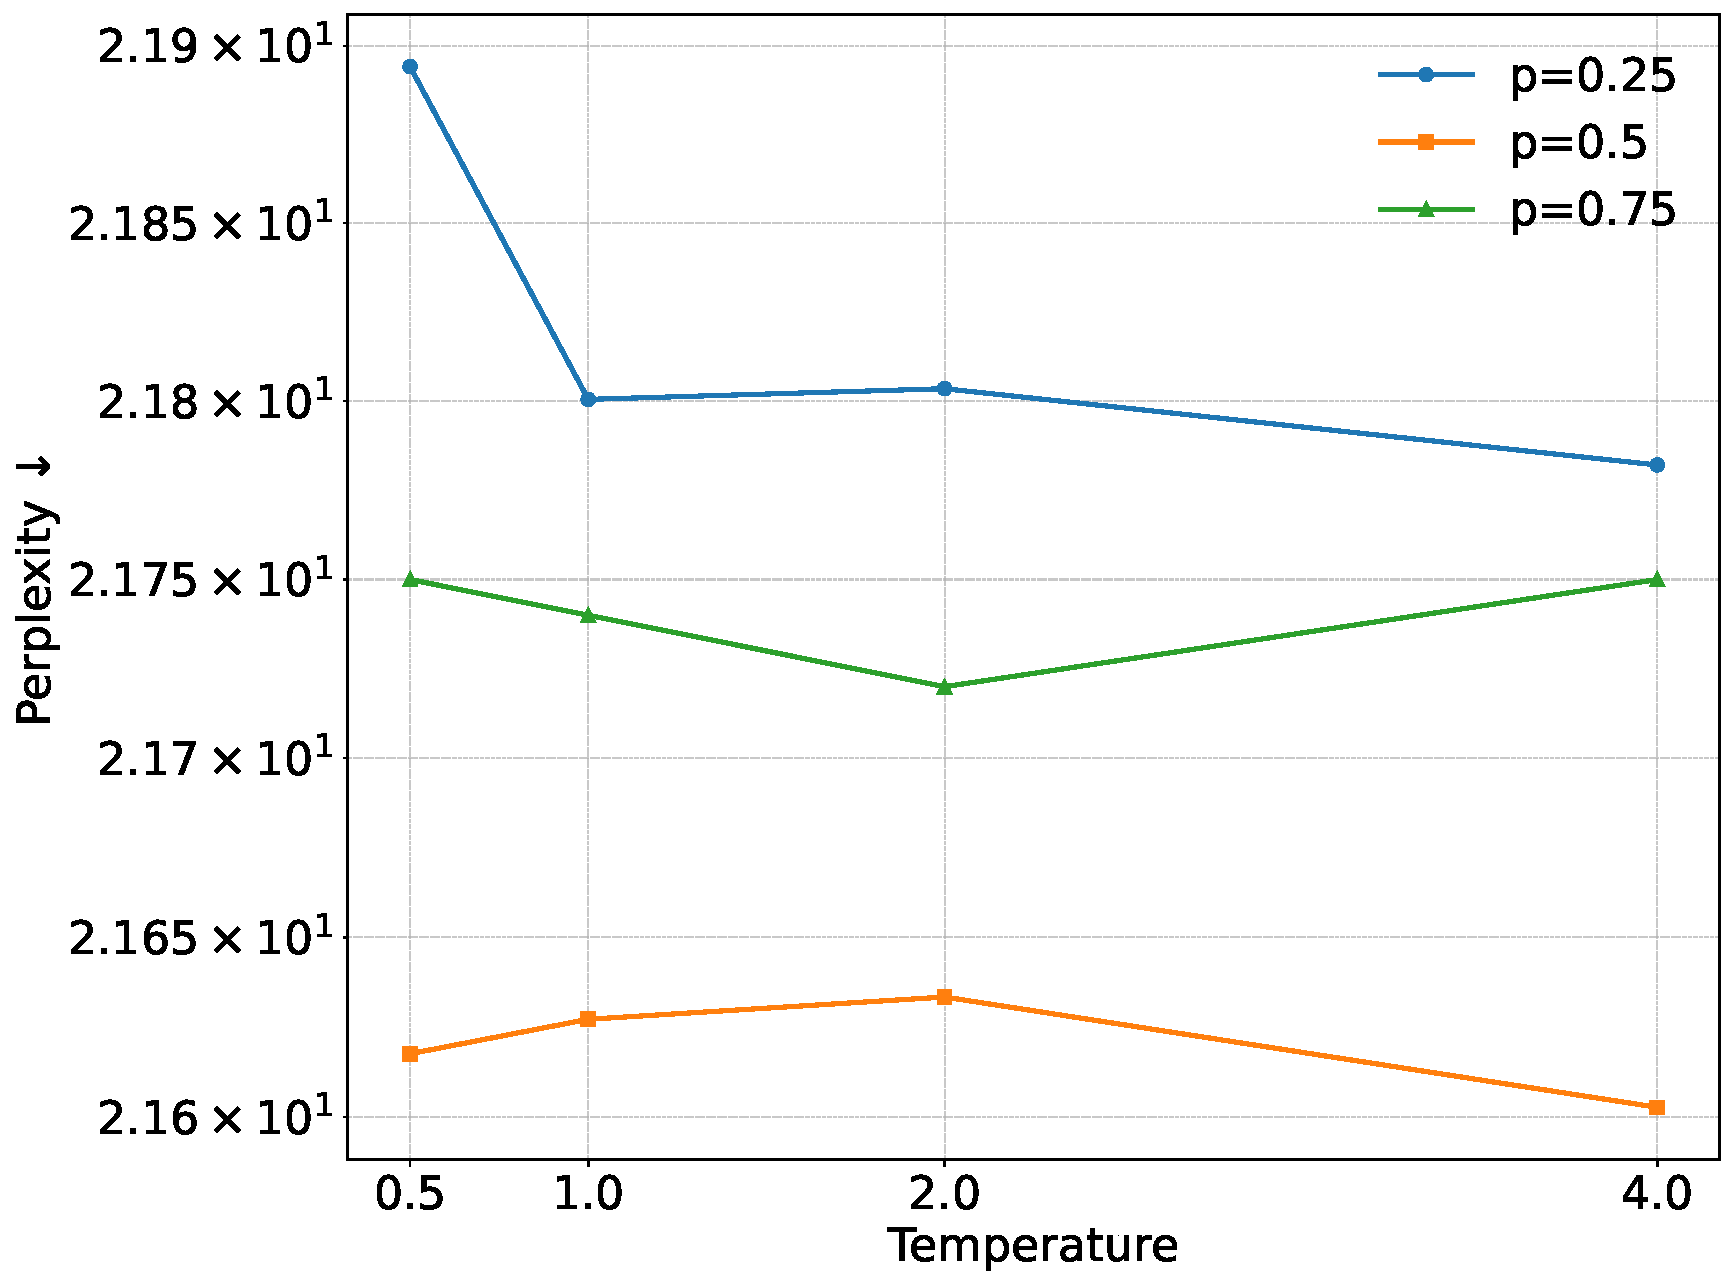
\includegraphics[width=\linewidth]{figs/sampling_ratio_and_damping_temperature.pdf} 
        \caption{不同采样比例 $p$ 与阻尼温度 $\tau$ 下的评估困惑度对比。}
        \label{fig:sampling-ratio-damping-temperature-sweep}
    \end{minipage}
    \hfill 
    \begin{minipage}[b]{0.45\textwidth}
        \centering
        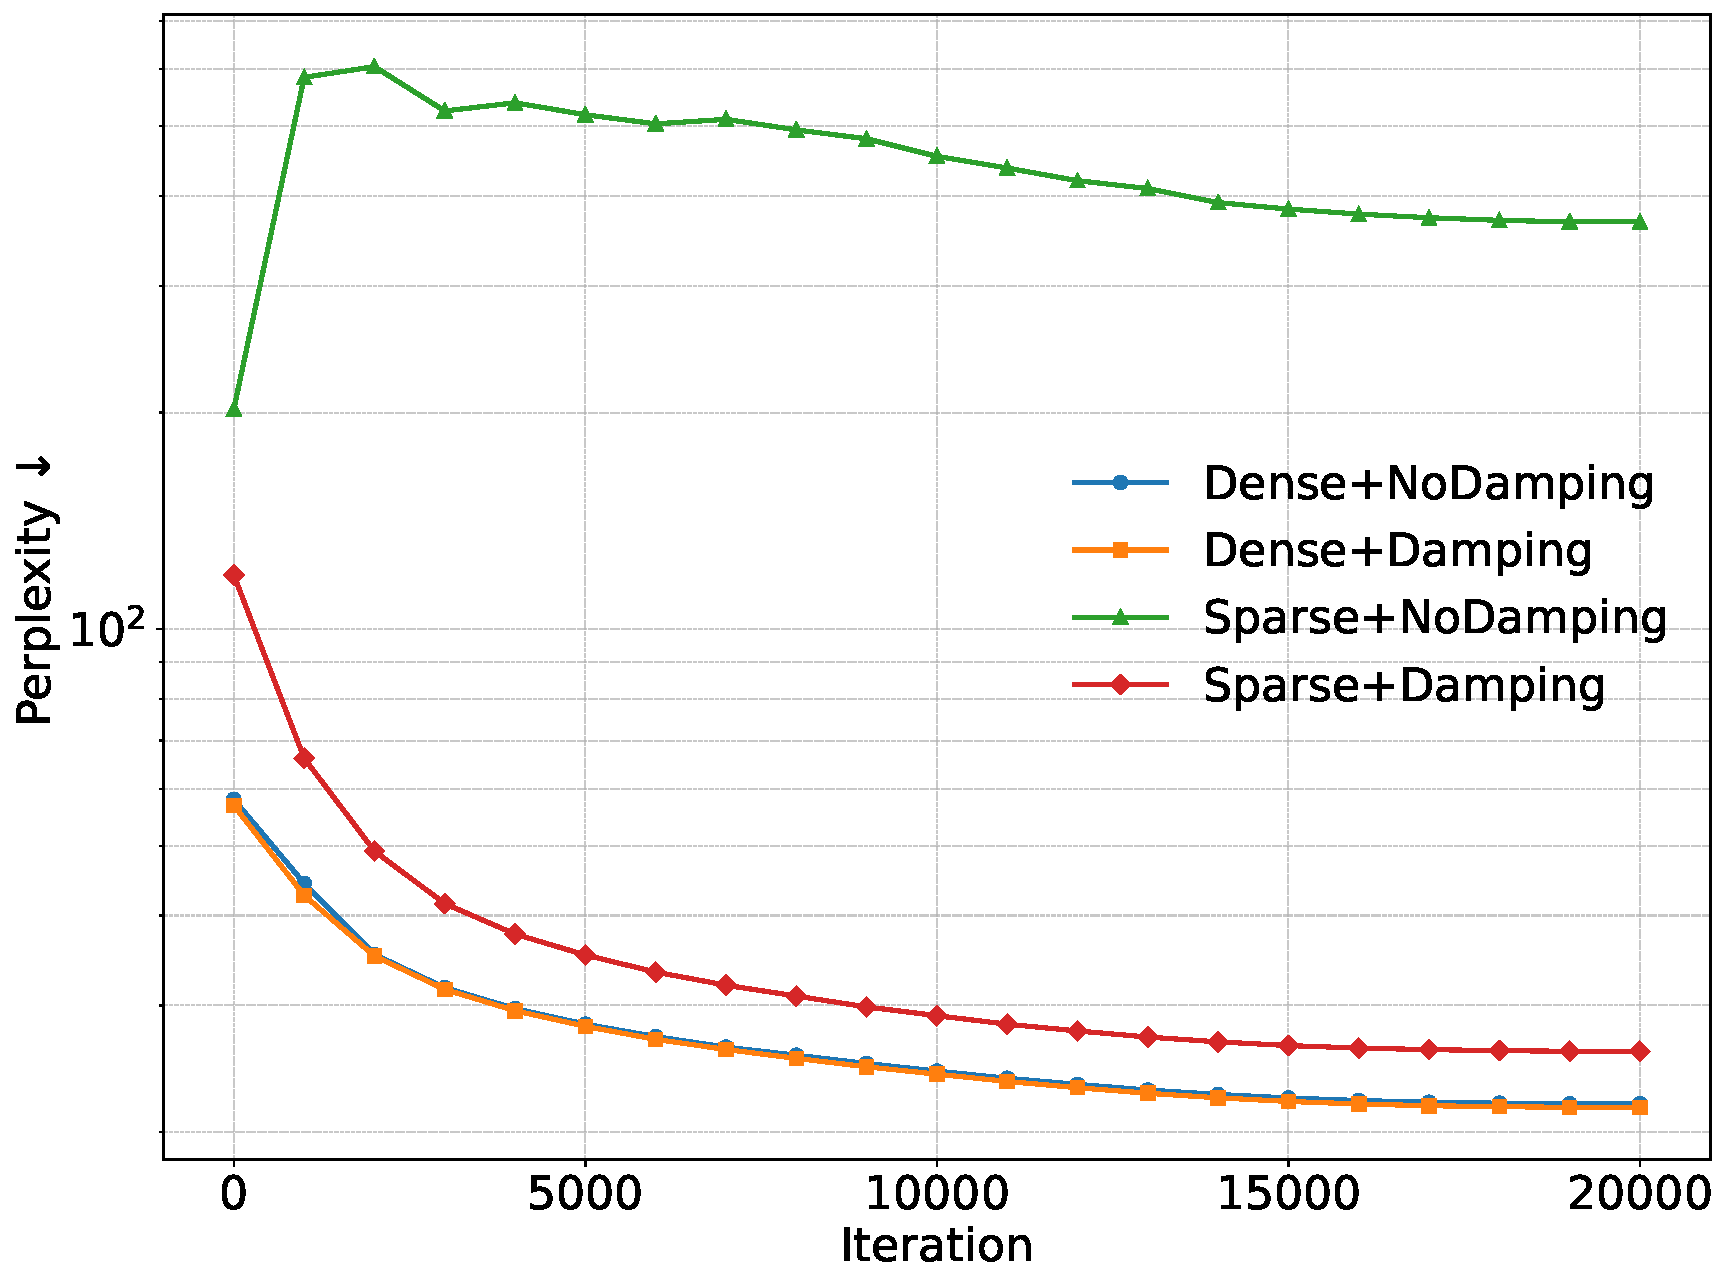
\includegraphics[width=\linewidth]{figs/dense_vs_sparse_momentum_update.pdf} 
        \caption{在 C4 数据集上训练 20,000 次迭代时，稠密与稀疏动量更新（含/不含阻尼）的训练困惑度对比。 }
        \label{fig:dense-vs-sparse-momentum-update}
    \end{minipage}
\end{figure}




% \begin{figure}
% % \vskip -0.1in
% \begin{center}
% 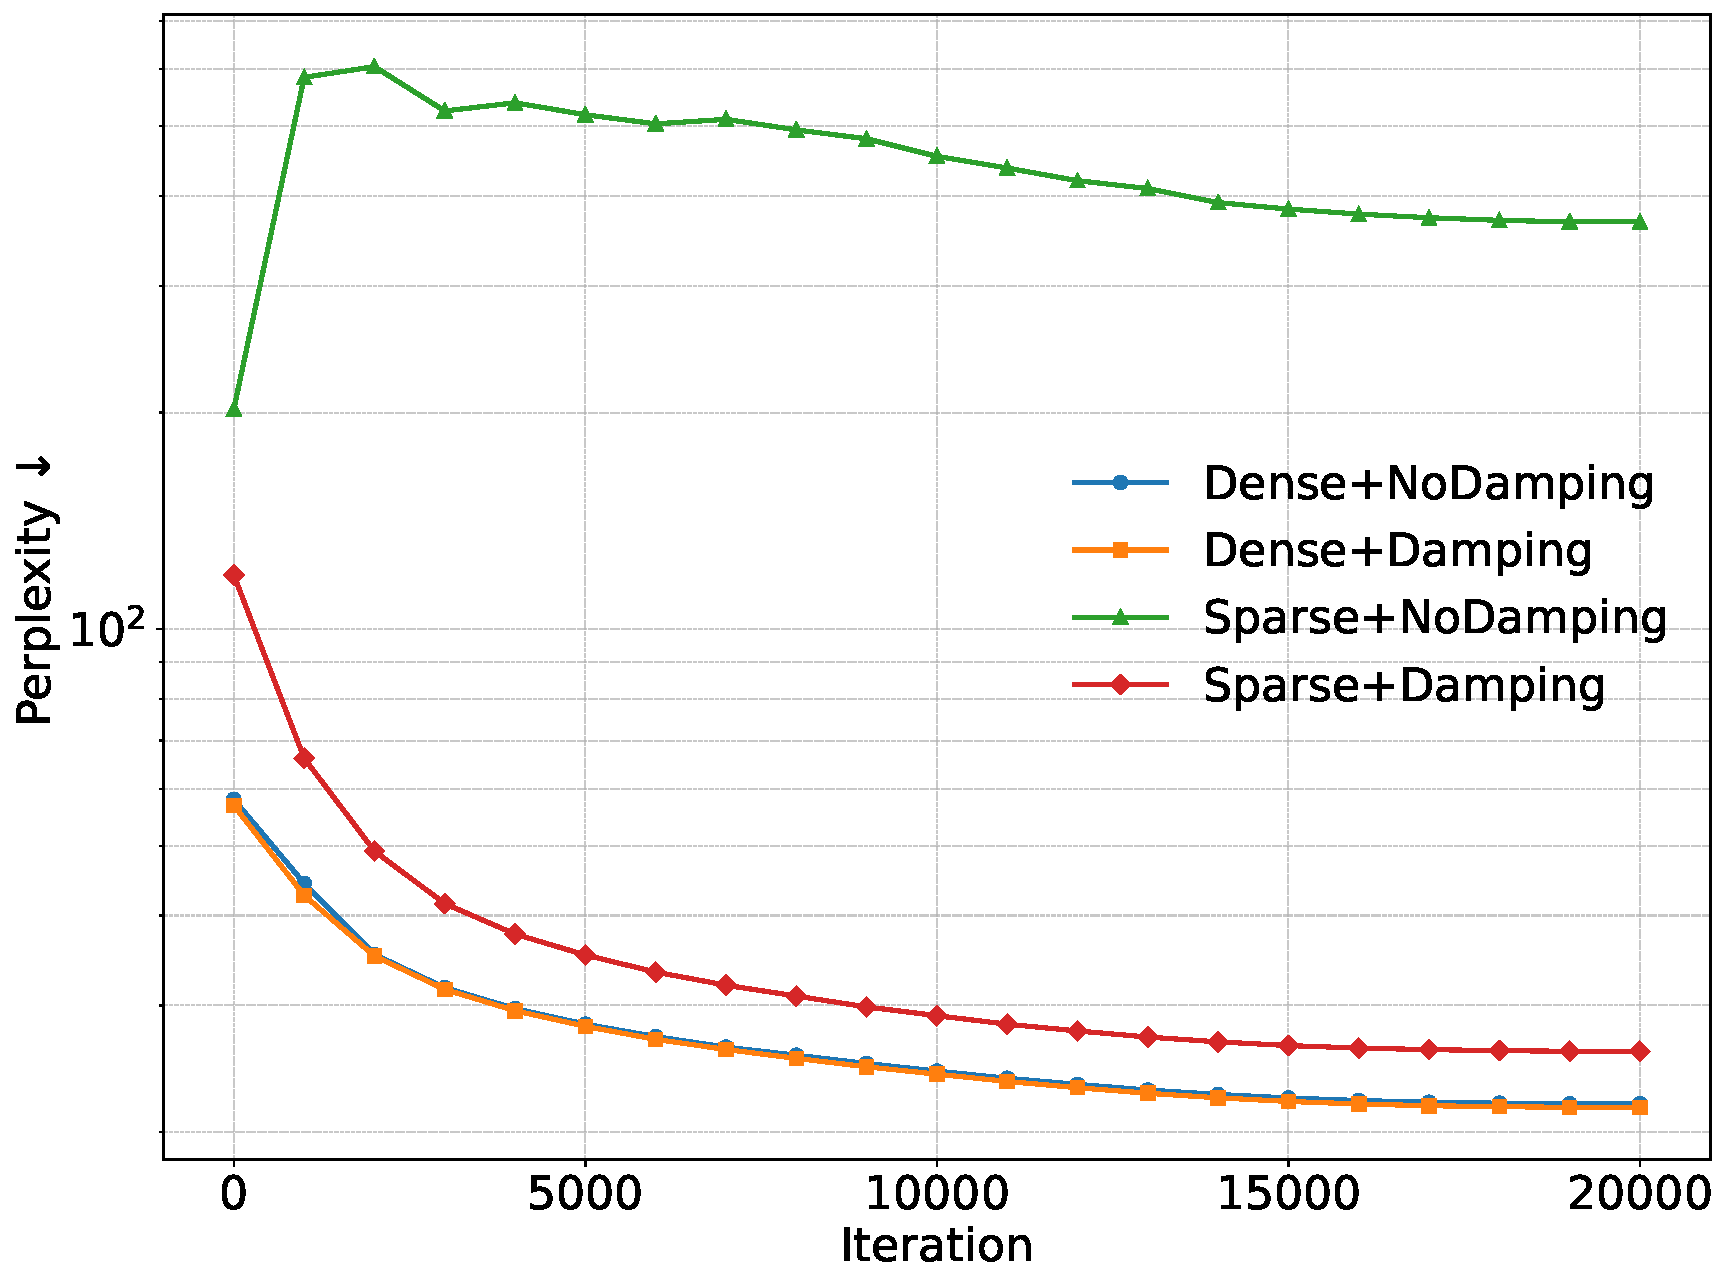
\includegraphics[width=0.5\columnwidth]{figs/dense_vs_sparse_momentum_update.pdf}
% \end{center}
% \caption{
% 在 C4 数据集上训练 20,000 次迭代时，稠密与稀疏动量更新（含/不含阻尼）的训练困惑度对比。 
% % 进一步细节见附录 \ref{subsec:sparse-vs-dense-momentum-update}。 
% }
% \label{fig:dense-vs-sparse-momentum-update}
% % \vskip -0.3in
% \end{figure}


\subsection{采样比例与阻尼温度}
为确定最优采样比例 $p$ 与阻尼温度 $\tau$，我们测试了 $p \in \{0.25, 0.5, 0.75\}$ 与 $\tau \in \{ 0.5, 1.0, 2.0, 4.0\}$。如图~\ref{fig:sampling-ratio-damping-temperature-sweep} 所示，在所有温度下，$p=0.5$ 均优于其他取值。另一方面，结果对温度不太敏感，因此我们在全部实验中采用 $\tau=2.0$。


% \begin{figure} 
% % \vskip -0.1in
% \begin{center}
% 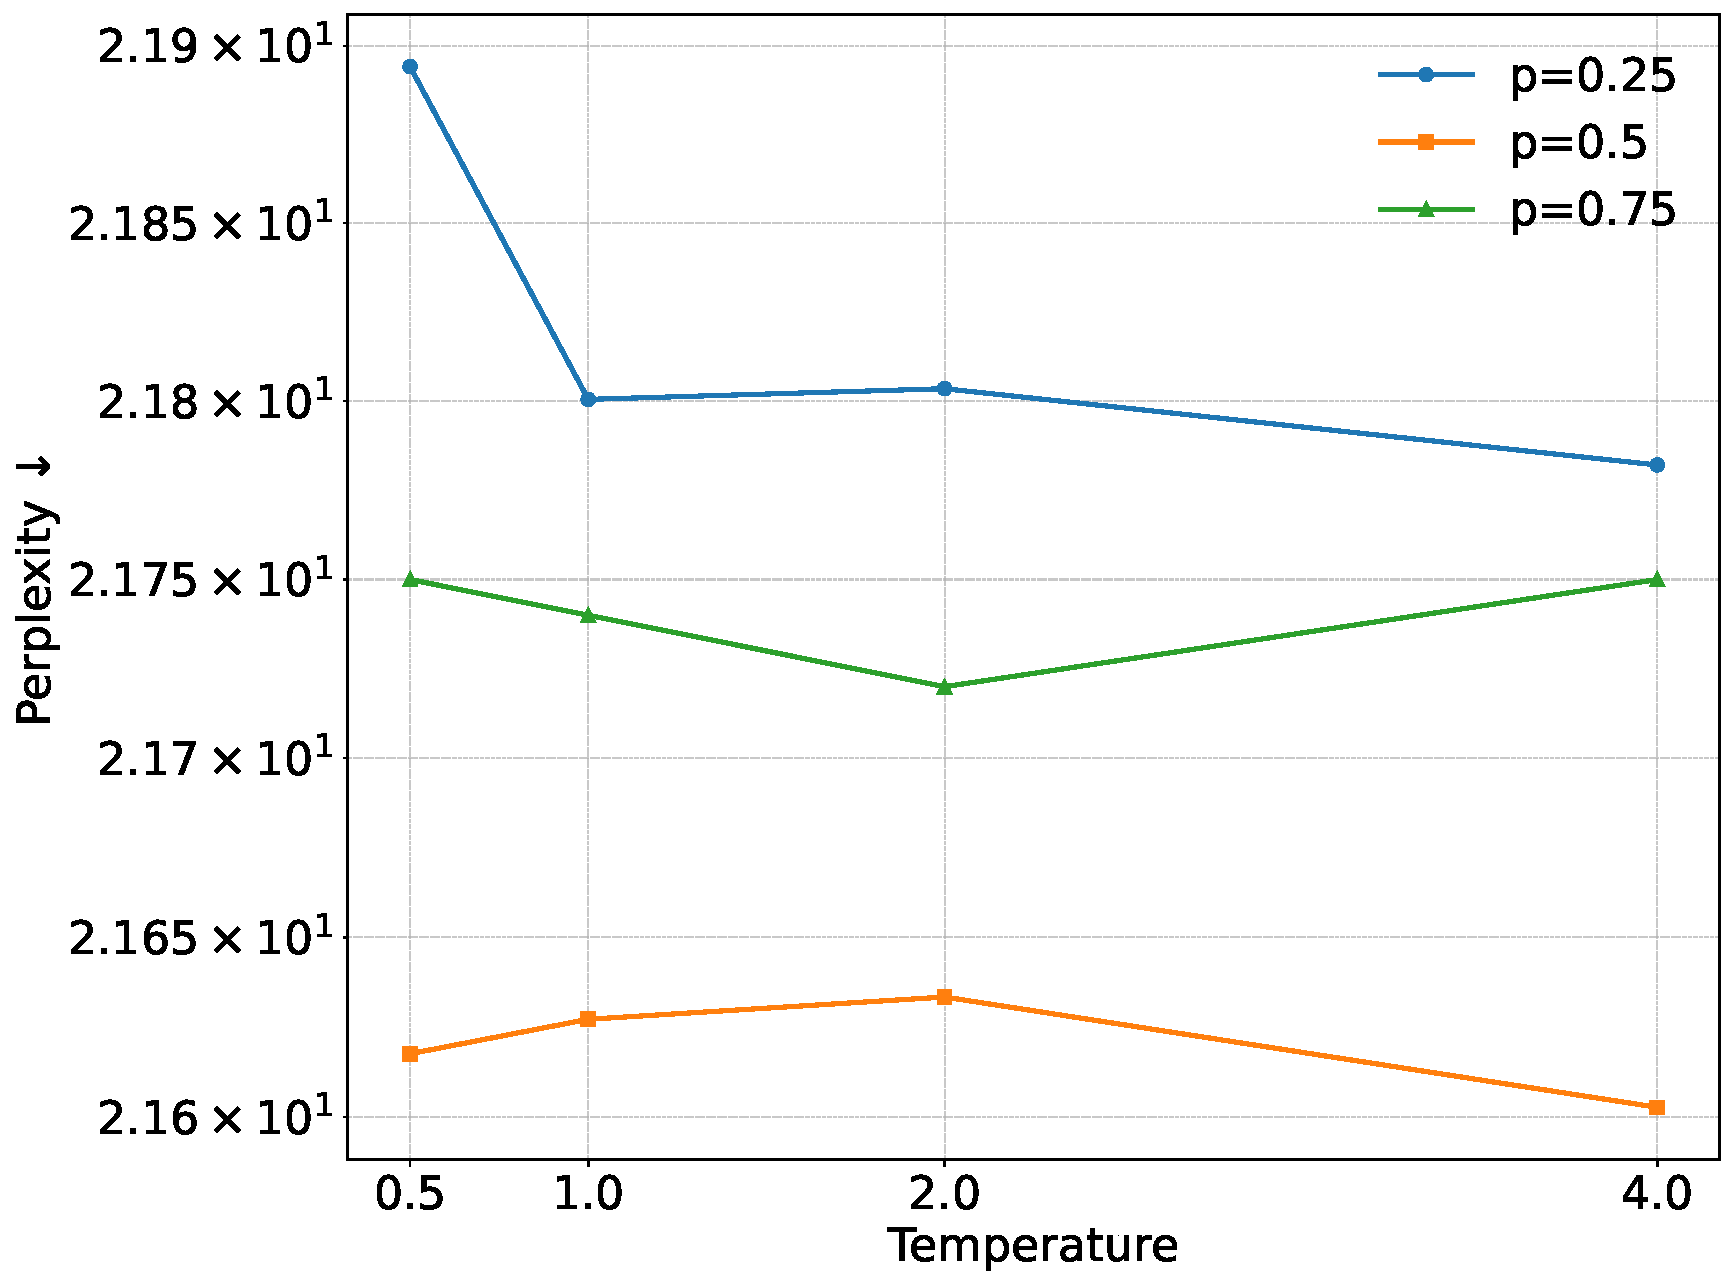
\includegraphics[width=0.5\columnwidth]{figs/sampling_ratio_and_damping_temperature.pdf}
% \end{center}
% \caption{
% 不同采样比例 $p$ 与阻尼温度 $\tau$ 下的评估困惑度对比。
% }
% \label{fig:sampling-ratio-damping-temperature-sweep}
% \end{figure}



\begin{figure} 
% \vskip -0.1in
\begin{center}
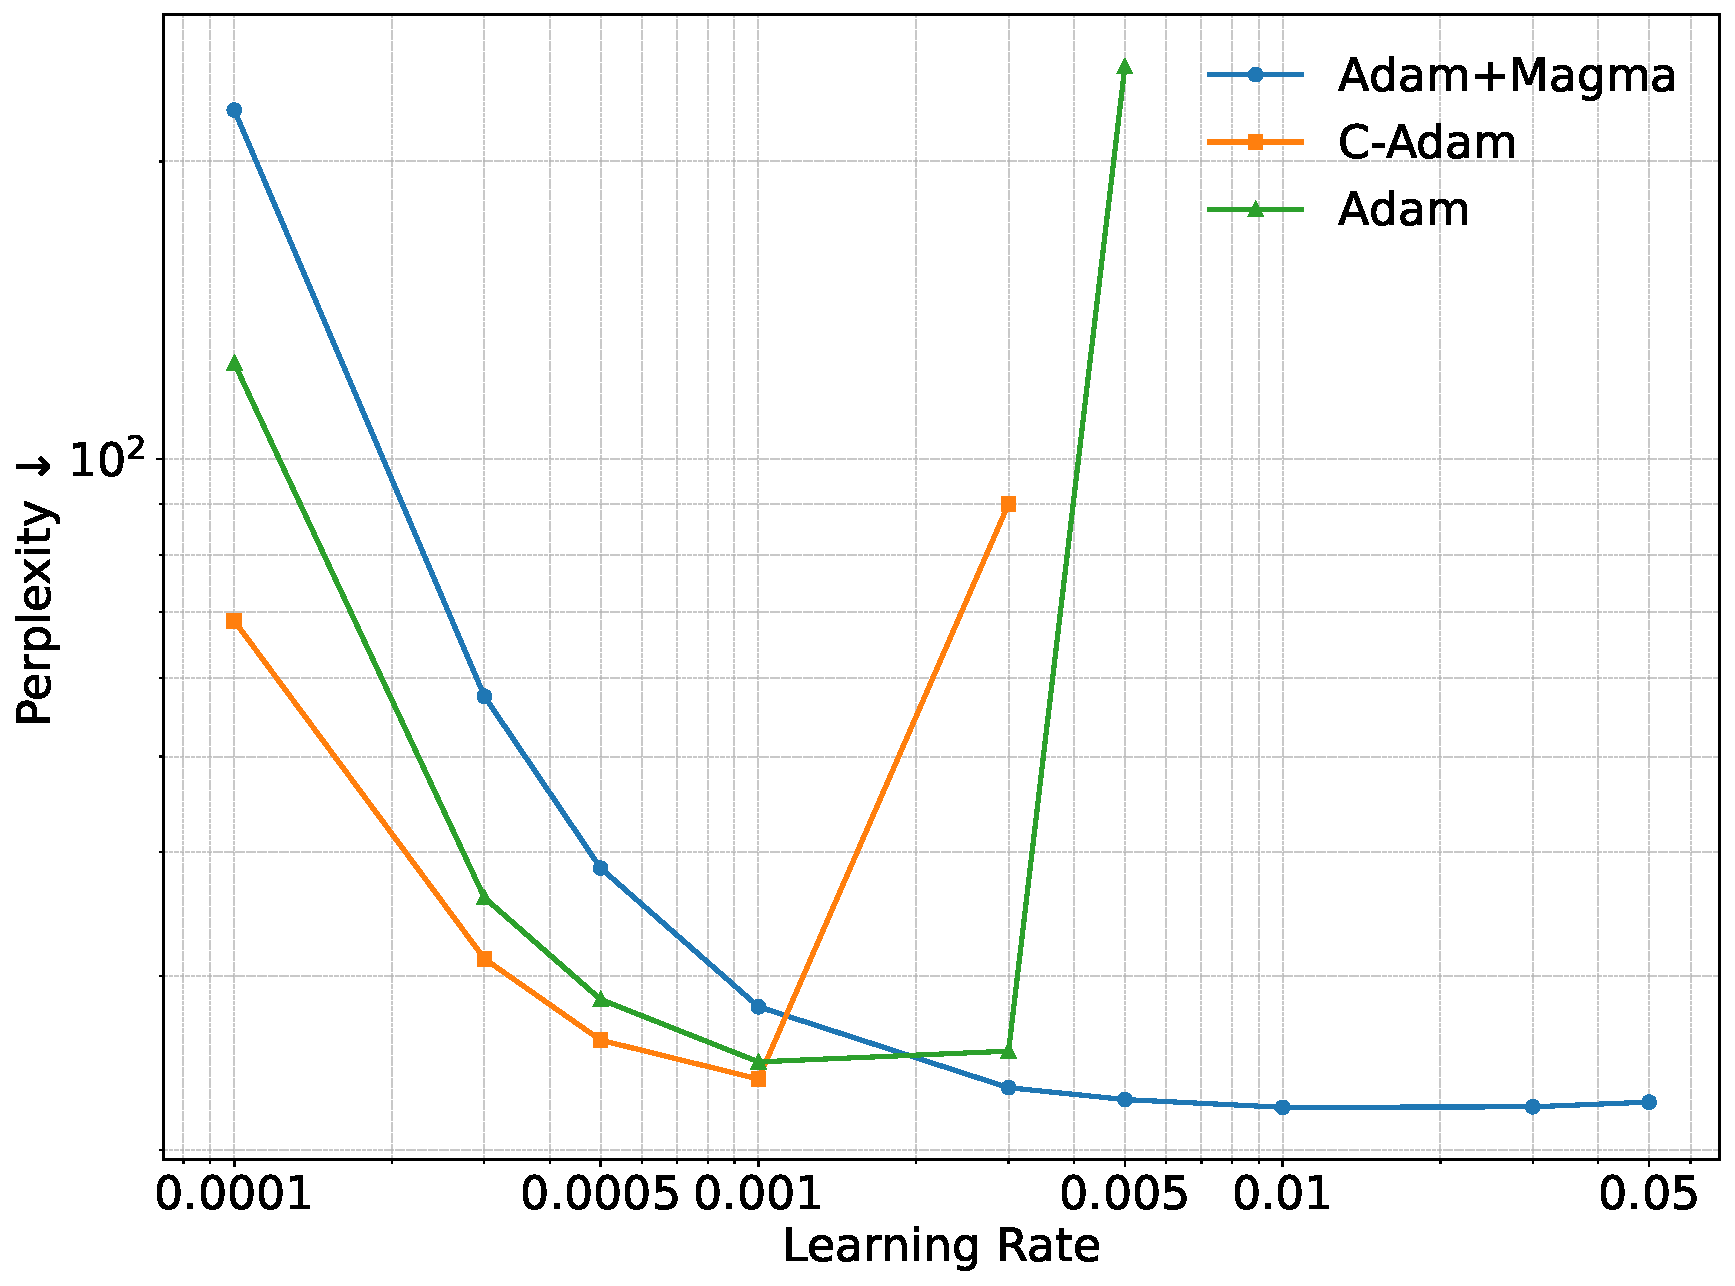
\includegraphics[width=0.5\columnwidth]{figs/learning_rate_sensitivity.pdf}
\end{center}
\caption{学习率敏感性分析。与最优窗口较窄的 Adam 与 C-Adam 不同，Adam+Magma 保持稳定性能，表现出在显著更宽超参数范围内的稳定性。}
\label{fig:learning-rate-sensitivity}
% \vskip -0.2in
\end{figure}




\subsection{稀疏与稠密动量更新对比}
\label{subsec:sparse-vs-dense-momentum-update}
我们在学习率 0.001 下比较了四种设置。结果显示稠密与稀疏更新方法存在关键差异。如图~\ref{fig:dense-vs-sparse-momentum-update} 所示，稠密基线（无论是否阻尼）都能持续保持稳健收敛并达到最低困惑度。相比之下，不带阻尼的稀疏动量更新表现出严重不稳定性：困惑度急剧升高并在 20,000 次迭代中维持高位。尽管引入阻尼后模型趋于稳定，其轨迹仍明显落后于稠密更新基线。







\subsection{学习率敏感性} 如图~\ref{fig:learning-rate-sensitivity} 所示，Adam+Magma 相较基线优化器对学习率变化更具鲁棒性。C-Adam 与 Adam 对学习率较敏感——当学习率偏离约 0.001–0.003 时，困惑度会明显恶化——而 Adam+Magma 在更宽范围内保持稳定。尤其是在高达 0.05 的区间内仍有效，而其他优化器在该区间难以收敛。这说明 Adam+Magma 可降低对精细超参数调节的依赖，为资源受限实验提供更高可靠性。





\end{document}
